\section{The normal model}
\begin{slide}\slidetitle{The normal model}
\tableofcontents[sectionstyle=show/hide,subsectionstyle=show/shaded/hide]

\end{slide}
\subsection{Normal problems}\begin{slide}\slidetitle{Normal model}
Sample
$$
x_1,\ldots,x_n
$$
from a normal $\mathcal{N}(\mu,\sigma^2)$ distribution

\centerline{\includegraphics[height=\textwidth,width=5truecm,angle=270]{figures/normalsample.ps}}

\end{slide}\begin{slide}
\slidetitle{Inference on $(\mu,\sigma)$ based on this sample}

\begin{itemize}
\item Estimation of \RedOrange{[transforms of]} $(\mu,\sigma)$ 
\pause
\item Confidence region \RedOrange{[interval]} on $(\mu,\sigma)$
\pause
\item Test on $(\mu,\sigma)$ and comparison with other samples
\end{itemize}

\end{slide}
\begin{slide}\slidetitle{Datasets}
\begin{block}{\BurntOrange{\bfseries {Larcenies {\sf =normaldata}}}}
\begin{columns}
\column{.45\textwidth}
Relative changes in reported
larcenies between 1991 and 1995 (relative to 1991)
for the $90$ most populous US counties {\em (Source: FBI)}
\column{.45\textwidth}
%\only<1>{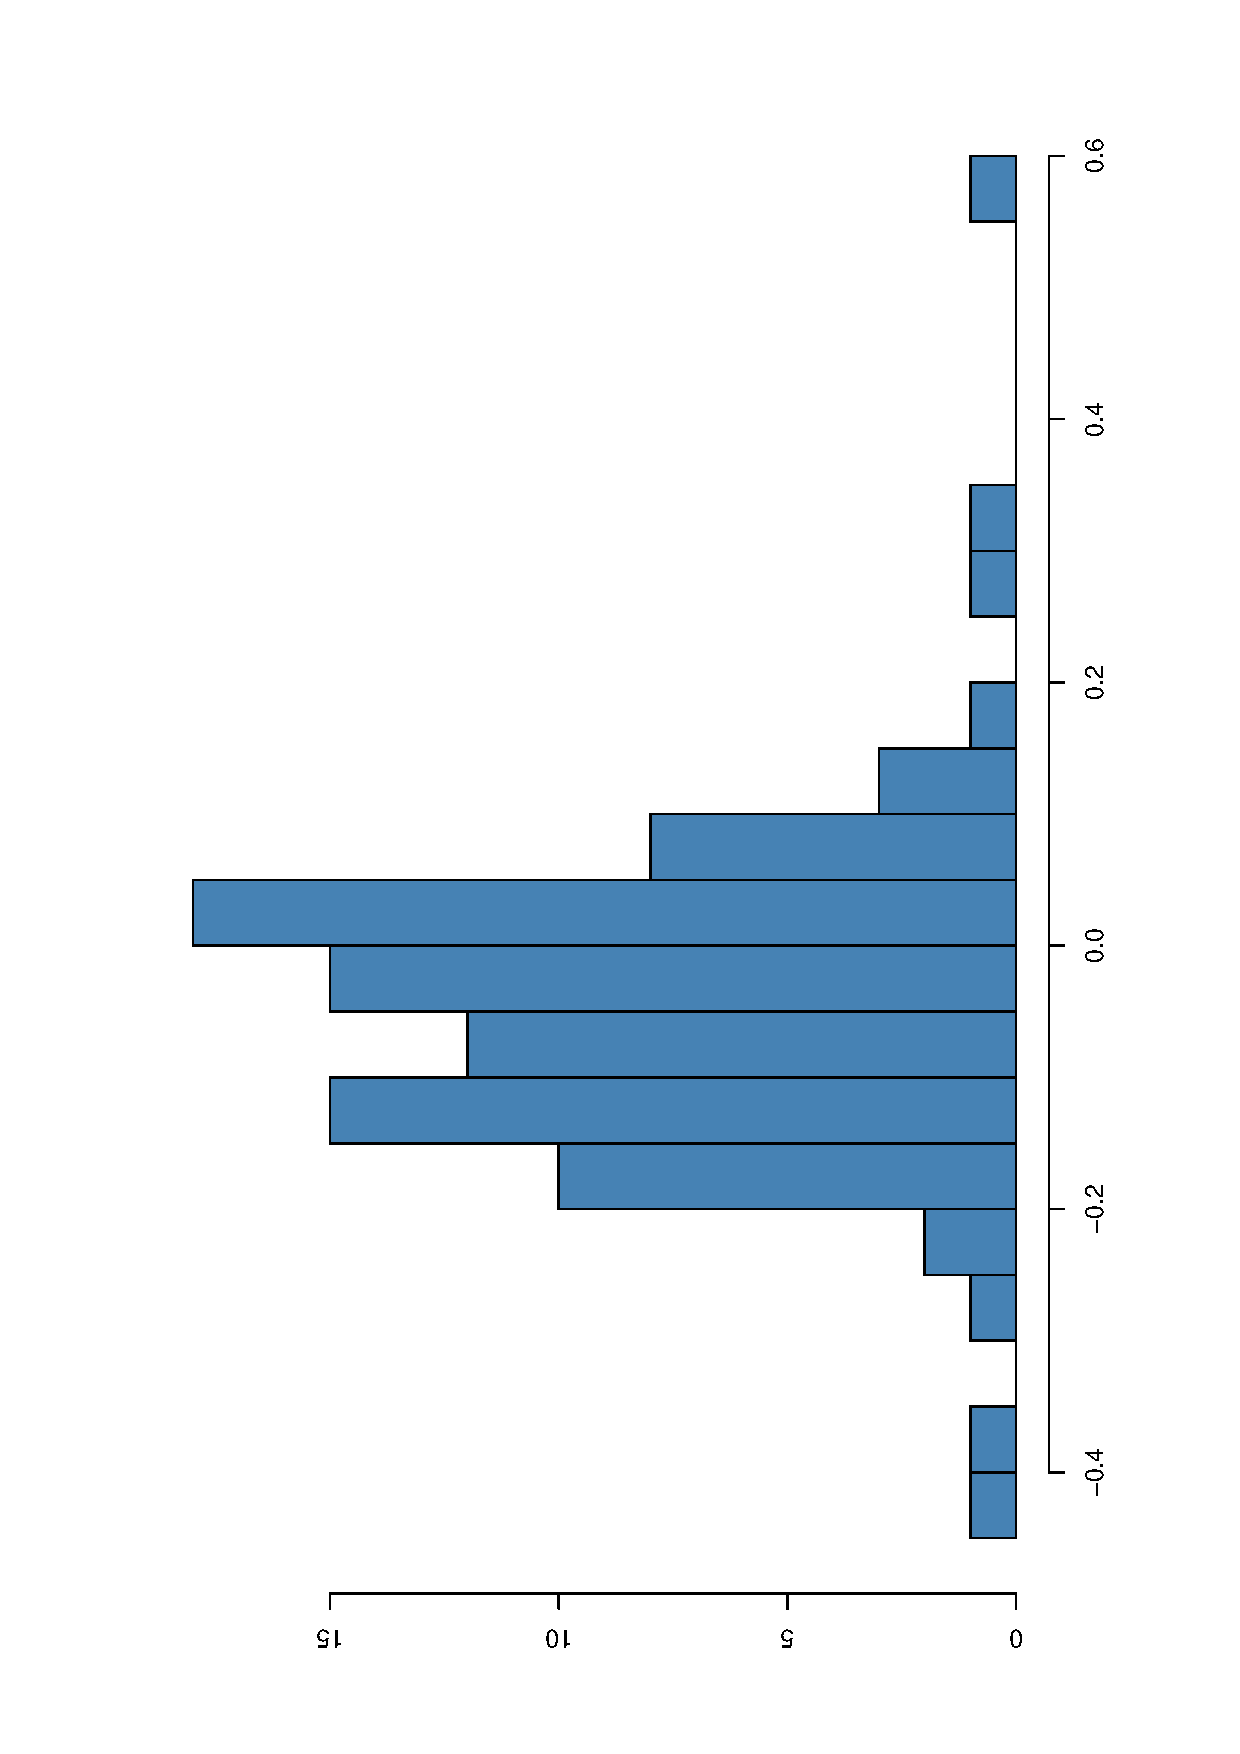
\includegraphics[height=5truecm,width=5truecm,angle=270]{figures/normdata}}
%\only<2>{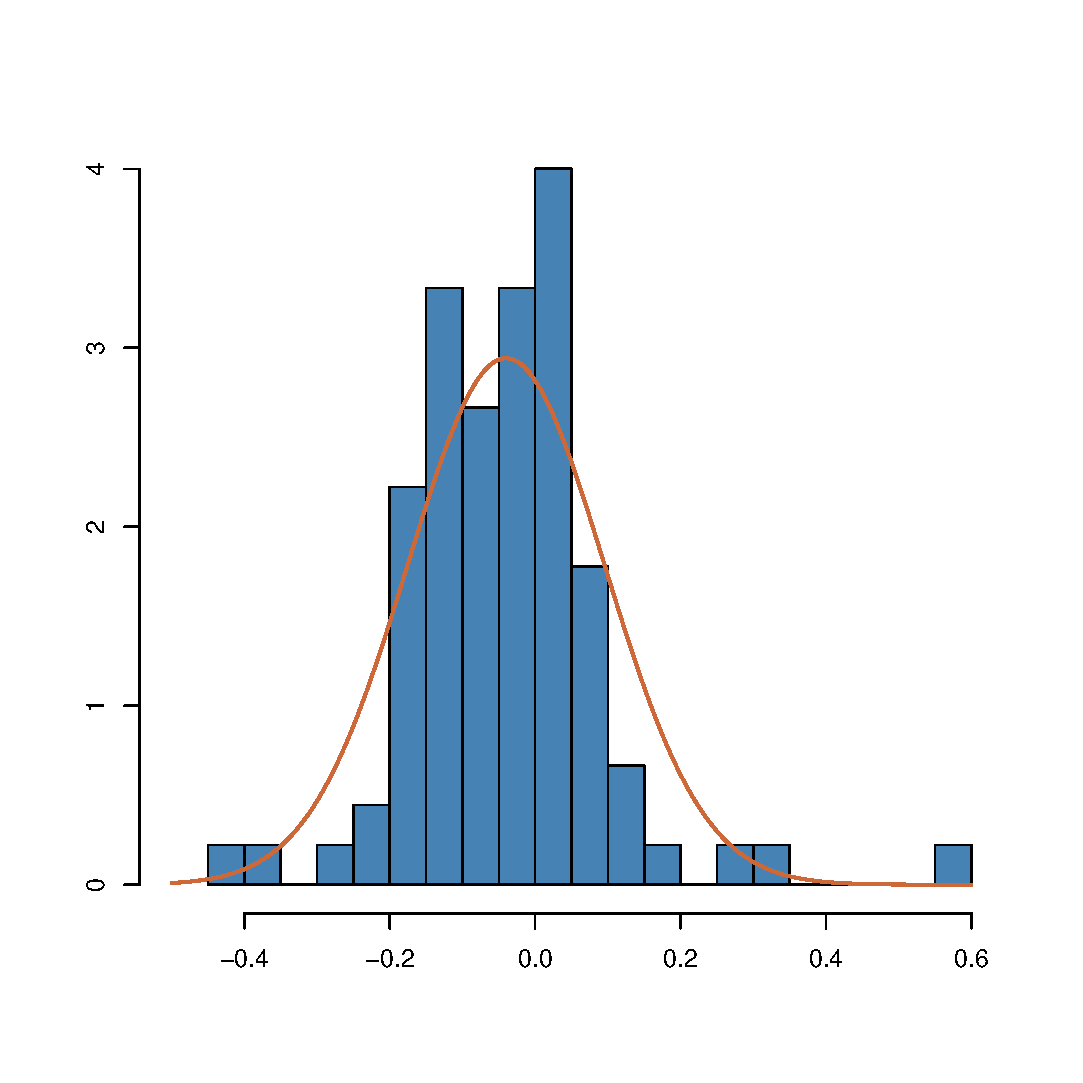
\includegraphics[height=5truecm,width=5.3truecm]{figures/normdataplus}}
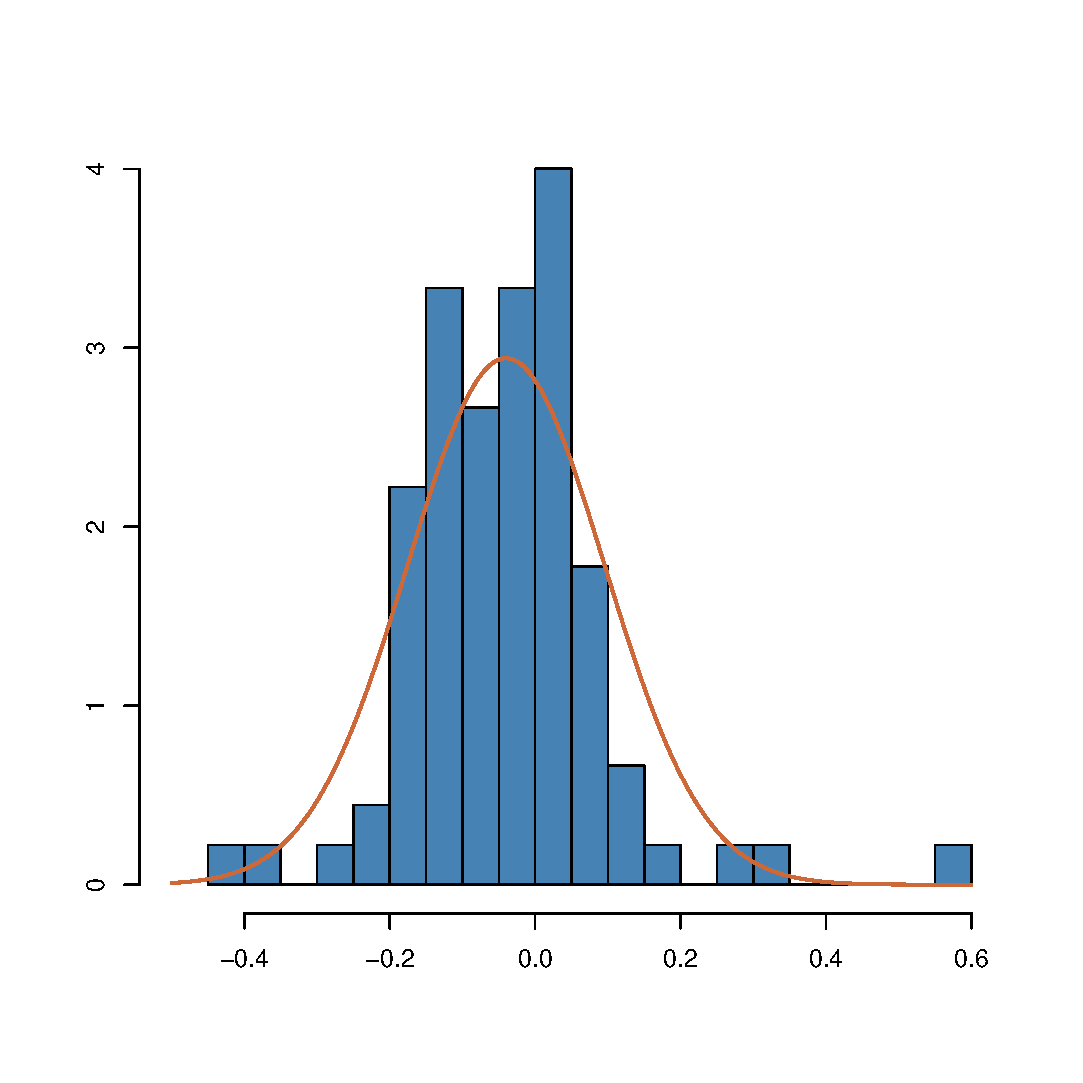
\includegraphics[height=5truecm,width=5.3truecm]{figures/normdataplus}
\end{columns}
\end{block}
\end{slide}
\begin{slide}
\begin{block}{\BurntOrange{\bfseries {Cosmological background {\sf =CMBdata}}}}
\begin{columns}
\column{.5\textwidth}
Spectral representation of the ``cosmological microwave background" (CMB),
i.e.~ electromagnetic radiation from photons back to $300,000$ years
after the Big Bang, expressed as difference in apparent temperature from the mean
temperature
\column{.45\textwidth}
\only<1>{\includegraphics[height=5truecm,width=5truecm,angle=270]{figures/CMBcol}}

\end{columns}
\end{block}
\end{slide}
\begin{slide}
\begin{block}{\BurntOrange{\bfseries {Cosmological background {\sf =CMBdata}}}}
Normal estimation
\only<1>{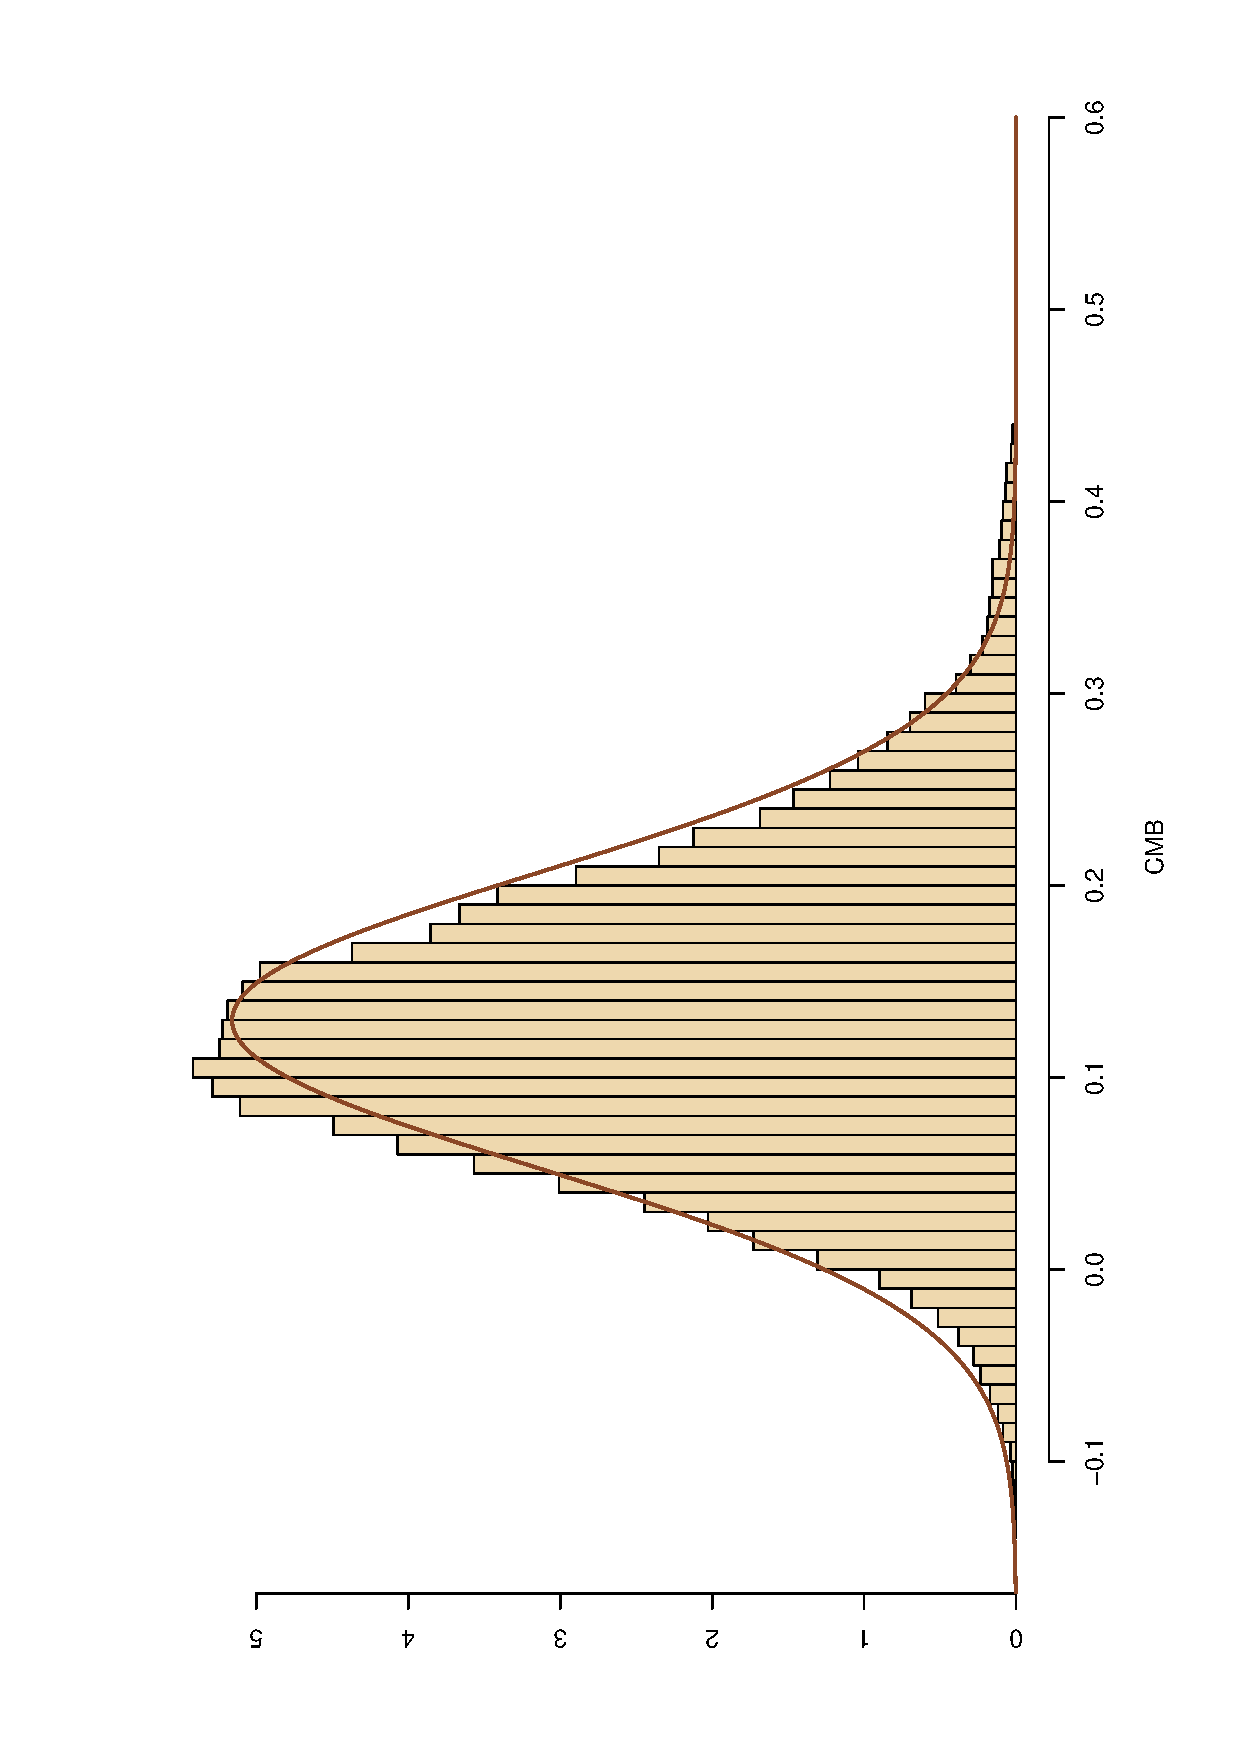
\includegraphics[height=5truecm,width=5truecm,angle=270]{figures/CMBnor}}
\end{block}
\end{slide}
\begin{slide}
\begin{block}{\BurntOrange{\bfseries {Cosmological background {\sf =CMBdata}}}}
Normal estimation
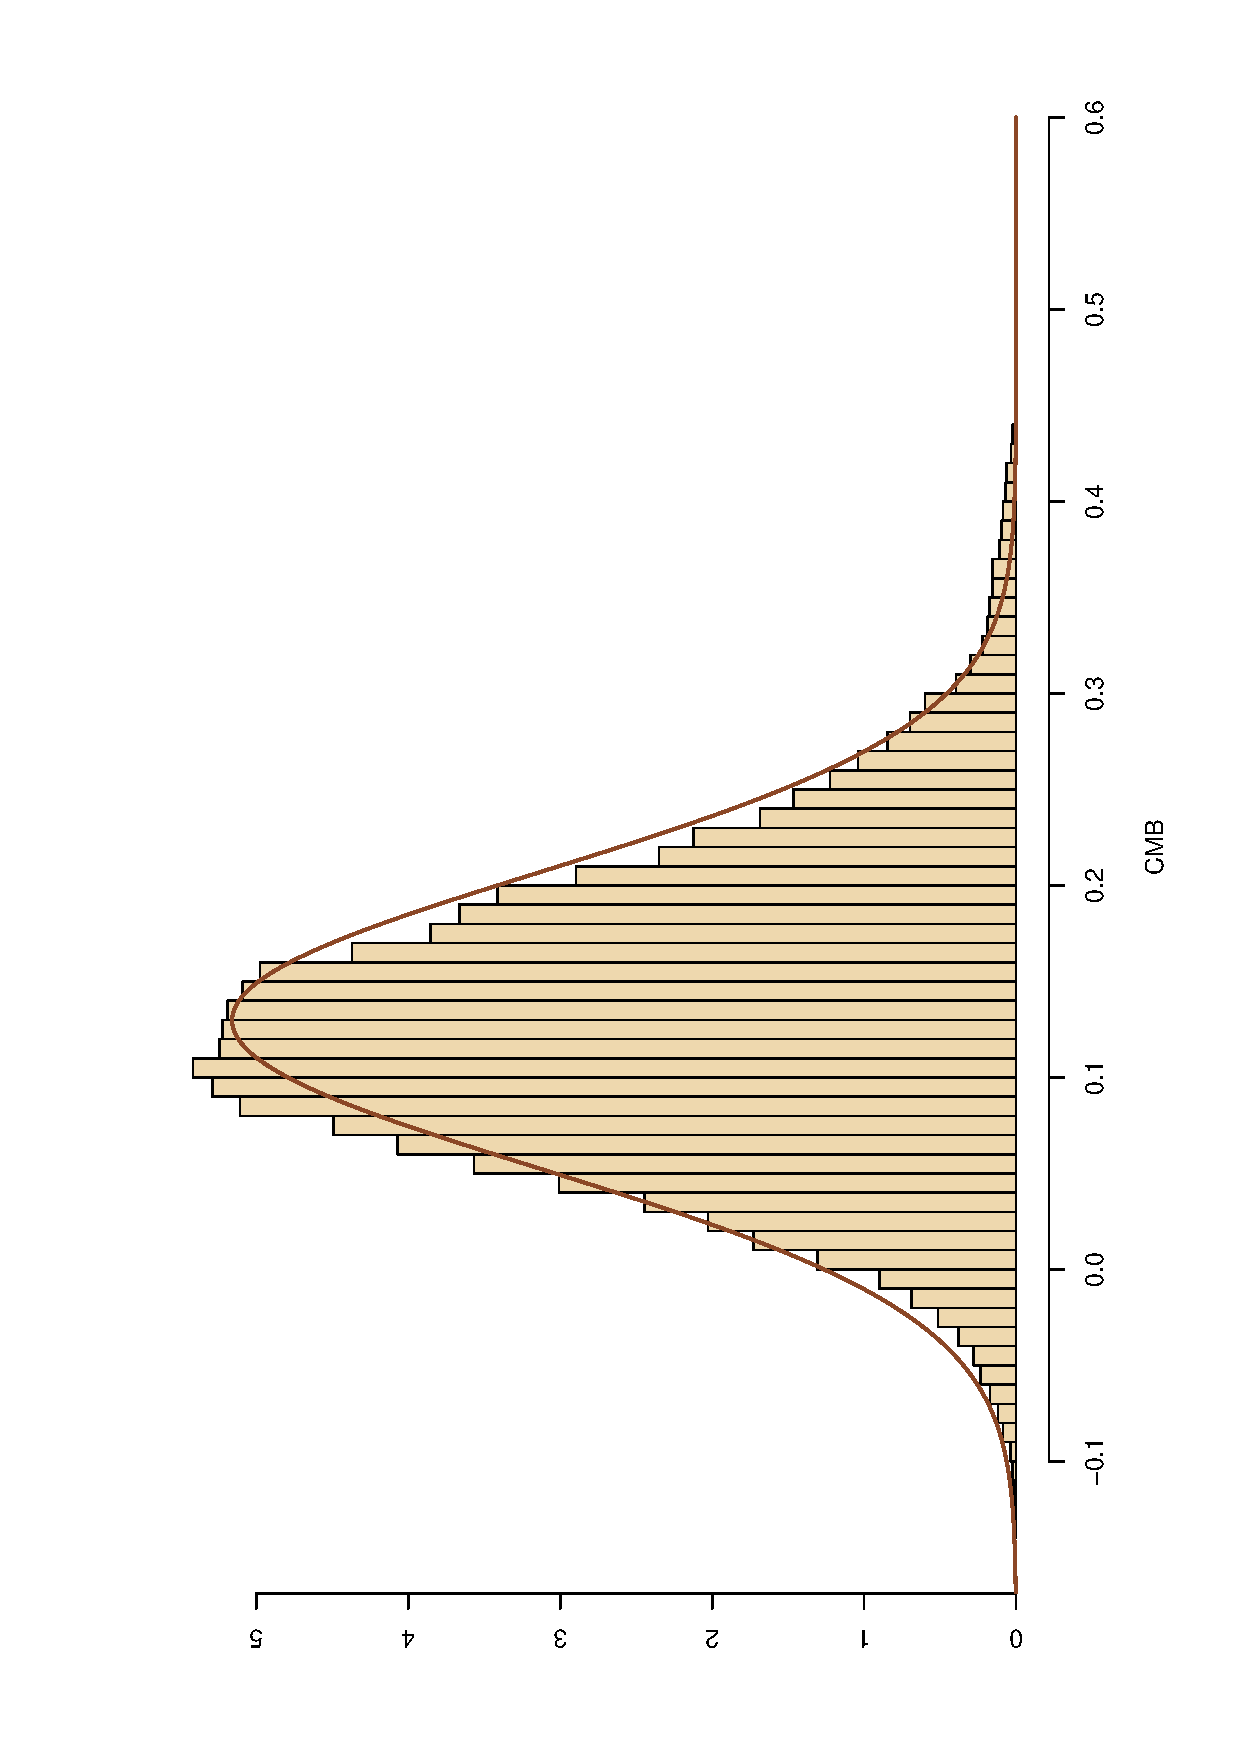
\includegraphics[height=5truecm,width=5truecm,angle=270]{figures/CMBnor}
\end{block}
\end{slide}

\subsection{The Bayesian toolbox}\begin{slide}\slidetitle{The Bayesian toolbox}

\centerline{\BurntOrange{\fbox{\bf Bayes theorem = Inversion of probabilities}}}

\bigskip
\pause
If $A$ and $E$ are events such that $P(E)\ne 0$, $P(A|E)$ and $P(E|A)$ are related by
{\Brown{
\begin{eqnarray*}
P(A|E) &=& {P(E|A) P(A) \over P(E|A) P(A) + P(E|A^c) P(A^c)}\\
&=& {P(E|A) P(A) \over P(E)} 
\end{eqnarray*}
}}

\end{slide}
\begin{slide}
\slidetitle{\Blue{\sf Who's Bayes?}}

\begin{block}{\BrickRed{{\bf Reverend Thomas Bayes (ca. 1702--1761)}}}
\begin{columns}\column{.5\textwidth}
Presbyterian minister in Tunbridge Wells (Kent) from 1731, son of Joshua Bayes, nonconformist minister.
Election to the {\em Royal Society} based on a tract of 1736 where he defended the views
and philosophy of Newton.

\column{.4\textwidth}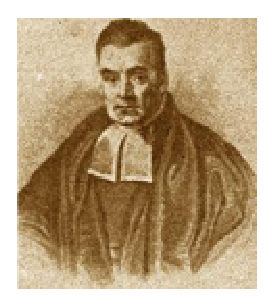
\includegraphics[height=4truecm]{figures/TBayes}
\end{columns}

\medskip
\pause
Sole probability paper, {\em ``Essay Towards Solving a Problem in the Doctrine of Chances"},
published posthumously in 1763 by Pierce
and containing the seeds of {\em Bayes' Theorem}.%Philosophical Transactions of the Royal Society of London.
\end{block}

\end{slide}
\begin{slide}
\slidetitle{New perspective}
\begin{itemize}
\item {\it Uncertainty} on the parameters $\theta$ of a model 
modeled through a {\it probability} distribution $\pi$ on $\Theta$, 
called {\it prior distribution}

\pause
\item {\it Inference} based on the distribution of $\theta$ conditional 
on $x$, $\pi(\theta|x)$, called {\it posterior distribution}
{\Brown{
\[
\pi(\theta|x) = {f(x|\theta) \pi(\theta) \over \int f(x|\theta) 
     \pi(\theta) \,d\theta}\ .
\]
}}
\end{itemize}

\end{slide}\begin{slide}
\slidetitle{Bayesian model}

A Bayesian statistical model is made of 
\begin{enumerate}
\item a likelihood \[{\Red{ f(x|\theta), }}\]
\pause and of 
\item a prior distribution on the parameters, \[{\Red{ \pi(\theta)\,. }}\]
\end{enumerate}

\end{slide}\begin{slide}
\slidetitle{Justifications}

\begin{itemize}
\item Semantic drift from unknown $\theta$ to random $\theta$
\pause
\item Actualization of information/knowledge on $\theta$ by extracting
      information/knowledge on $\theta$ contained in the observation $x$
\pause

\item Allows incorporation of imperfect/imprecise information in the decision process
\pause

\item Unique mathematical way to condition upon the observations 
     (conditional perspective) 
%\pause
%\item Penalization factor
\end{itemize}

\end{slide}\begin{slide}
\debut[Normal illustration $(\sigma^2=1)$]

Assume
\Red{$$
\pi(\theta) = \exp \{-\theta\} \, \mathbb{I}_{\theta>0}
$$}
\pause Then
\Red{\begin{eqnarray*}
\pi(\theta|x_1,\ldots,x_n) &\mathbf{\propto}&
\exp \{-\theta\} \, \exp \{-n(\theta-\overline{x})^2 /2\} \, \mathbb{I}_{\theta>0}\\
&\mathbf{\propto}& \exp \left\{ -n\theta^2/2 + \theta(n\overline{x}-1) \right\} \, \mathbb{I}_{\theta>0}\\
&\mathbf{\propto}& \exp \left\{-n(\theta - (\overline{x}-1/n))^2/2\right\} \, \mathbb{I}_{\theta>0}
\end{eqnarray*}}
\fin

\end{slide}\begin{slide}
\debut[Normal illustration (2)]
Truncated normal distribution
\Brown{$$
\mathcal{N}^+((\overline{x}-1/n),1/n) 
$$}
\centerline{\includegraphics[height=.7\textwidth,width=4.5truecm,angle=270]{figures/truncnormal.ps}}
\fin

\end{slide}
%\subsubsection{Prior and posterior distributions}
\begin{slide}\slidetitle{Prior and posterior distributions}

Given $f(x|\theta)$ and $\pi(\theta)$, several distributions of interest:
   \begin{enumerate}
\item the {\it joint distribution} of $(\theta,x)$,
$$
     \varphi(\theta,x) = f(x|\theta)\pi(\theta)\,;
$$

\pause
\item the {\it marginal distribution} of $x$, 
{\Brown{
\begin{eqnarray*}
m(x) &=&  \int \varphi(\theta,x) \,d\theta \\
  &=& \int f(x|\theta) \pi(\theta) \,d\theta\,; 
\end{eqnarray*}
}}
\end{enumerate}

\end{slide}\begin{slide}
   \begin{enumerate}
   \setcounter{enumi}{2}
\item the {\it posterior distribution} of $\theta$,
{\Brown{
\begin{eqnarray*}
\pi (\theta |x) &=& {f(x|\theta ) \pi (\theta ) \over \int f(x|\theta ) 	 
\pi (\theta ) \,d\theta} \\
  &=&  {f(x|\theta ) \pi (\theta ) \over m(x)}\,; 
\end{eqnarray*}
}}
\item the {\it predictive distribution} of $y$, when $y\sim g(y|\theta,x)$,
{\Brown{
$$
  g(y|x) = \int g(y|\theta,x) \pi(\theta|x) d\theta \,.
$$
}}
    \end{enumerate}

\end{slide}\begin{slide}
\slidetitle{Posterior distribution center of to Bayesian inference}
{\RawSienna{
$$
\pi(\theta|x) \propto f(x|\theta)\,\pi(\theta)
$$
}}
\begin{itemize}
\item Operates  {\Red{\sf conditional}} upon the observations

\pause
\item Integrate simultaneously prior information/knowledge {\Red{and}} 
information brought by $x$

\pause
\item Avoids averaging over the {\Red{\sf unobserved}} values of $x$

\pause
\item \Black {\Red{\sf Coherent}} updating of the information available on $\theta$, independent of the
      order in which i.i.d.\ observations are collected

\pause
\item Provides a {\Red{\sf complete}} inferential scope and an unique motor of inference
\end{itemize}

\end{slide}\begin{slide}
\debut[Normal-normal case] 
Consider $x|\theta \sim {\cal N}(\theta,1)$ and $\theta\sim{\cal N}(a,10)$.
\begin{eqnarray*}
\pi(\theta|x) & \propto &  f(x|\theta) \pi(\theta) \propto \exp \left(-{(x-\theta)^2 \over 2} - {(\theta-a)^2 \over 20}\right) \\
              & \propto &  \exp\left(-{11 \theta^2 \over 20}+\theta (x+a/10) \right) \\
              & \propto & \exp\left(-{11 \over 20}\left\{\theta-((10x+a)/11)\right\}^2\right) 
\end{eqnarray*}
\pause and 
{\Brown{
\[
  \theta|x \sim{\cal N} \left( (10x+a) \big/ 11 , 10 \big/ 11 \right)
\]
}}
\fin

\end{slide}
%\subsubsection{Improper prior distributions}
\subsection{Prior selection}
\begin{slide}
\slidetitle{Prior selection}

\centerline{\BurntOrange{\fbox{\bf The prior distribution is the key to Bayesian inference}}}

\medskip
\pause{\MidnightBlue{{\bf But...}}}

In practice, it seldom occurs that the available prior 
information  is precise enough to lead to an exact 
determination of the prior distribution\\

\medskip\pause
\centerline{\MidnightBlue{\fbox{\bf There is no such thing as 
	{\it the} prior distribution!}}}

\end{slide}\begin{slide}
\slidetitle{Strategies for prior determination}

\small\begin{flushleft}
\begin{quote}
Ungrounded prior distributions produce\\
unjustified posterior inference.\\
---Anonymous, ca.~2006
\end{quote}
\end{flushleft}\normalsize

\pause
\begin{itemize}
\item Use a partition of $\Theta$ in sets (e.g., intervals), 
determine the probability of each set, and approach $\pi$
by an {\it histogram\/}
\pause
\item Select significant elements of
$\Theta$, evaluate their respective \like s and deduce a \like\
curve proportional to $\pi$
\pause
\item Use the {\it marginal distribution} of $x$,
$$
  m(x) = \int_\Theta f(x|\theta)\pi(\theta) \,d\theta
$$ 
\pause
\item Empirical and {\it \hier}\ Bayes techniques
\end{itemize}
\end{slide}
\begin{slide}[label=conju]\slidetitle{Conjugate priors}

Specific parametric family with analytical properties

\begin{block}{Conjugate prior}\label{def:3.1} \ A family $\CF$ of 
probability distributions on $\Theta$ is {\it conjugate}\ 
for a likelihood function $f(x|\theta)$ if, for every $\pi \in \CF$, 
the posterior distribution $\pi(\theta|x)$ also belongs to $\CF$.
\end{block}

\pause
\medskip
Only of interest when $\CF$ is {\it parameterised} :
switching from prior to posterior distribution is reduced 
to an {\BurntOrange{\sf updating}} of the corresponding parameters. 

\end{slide}\begin{slide}
\slidetitle{Justifications}

\begin{itemize}
\item Limited/finite information conveyed by $x$ 
\item Preservation of the structure of $\pi(\theta)$
\pause
\item Exchangeability motivations
\item Device of virtual past observations
\pause
\item Linearity of some estimators
\item But mostly... \pause \MidnightBlue{tractability and simplicity}
\pause
\item First approximations to adequate priors, backed up by robustness analysis
\end{itemize}

\end{slide}\begin{slide}
\slidetitle{Exponential families}

Sampling models of interest

\begin{block}{Exponential family} The family of distributions 
{\Brown{\[
f(x|\theta) = C(\theta) h(x) \exp\{R(\theta)\cdot T(x) \}
\]}}
is called an {\em \expo\ family of dimension $k$}.  When $\Theta 
\subset \BR^k$, $\CX \subset \BR^k$ and
{\Brown{\[
f(x|\theta) = h(x) \exp\{\theta\cdot x - \Psi(\theta) \},
\]}}
the family is said to be {\em natural}.
\end{block}

\end{slide}\begin{slide}
\slidetitle{Analytical properties of exponential families}
\begin{itemize}
\item Sufficient statistics (Pitman--Koopman Lemma)
\pause
\item Common enough structure (normal, Poisson, \&tc...)
\pause
\item Analyticity ($\BE[x] = \nabla \Psi(\theta)$, ...)
\pause
\item Allow for conjugate priors
\[\RedOrange{
  \pi(\theta|\mu,\lambda)=K(\mu,\lambda)\,e^{\theta.\mu-\lambda\Psi(\theta)}\qquad
  \lambda>0
}\]
\end{itemize}

\end{slide}\begin{slide}
\slidetitle{Standard exponential families}
{\MidnightBlue{
\begin{tabular}{|c|c|c|}
\hline
$\displaystyle \hfill f(x|\theta) \hfill$ & $\displaystyle \hfill \pi(\theta)
    \hfill$  & $\displaystyle \hfill \pi (\theta |x) \hfill$ \cr
\hline
$\displaystyle {\rm Normal}$ & ${\rm Normal}$ & \cr 
$\displaystyle \hfill {\cal N}(\theta,\sigma^2)$ & $\displaystyle \hfill
   {\cal N}(\mu,\tau^2)$ & 
    ${\cal N}(\rho (\sigma^2\mu+\tau^2 x),\rho \sigma^2\tau^2)$ \cr
 & & $\displaystyle \hfill \rho^{-1} = \sigma^2+\tau^2$ \cr
\hline
$\displaystyle \hfill {\rm Poisson}$ & ${\rm Gamma}$ & \cr
$\displaystyle \hfill {\cal P}(\theta)$ & $\displaystyle 
{\cal G}(\alpha,\beta)$ & $\displaystyle {\cal G}(\alpha +x,\beta +1)$ \cr
\hline
$\displaystyle \hfill {\rm Gamma}$ & ${\rm Gamma}$ & \cr
$\displaystyle \hfill {\cal G}(\nu ,\theta)$ & $\displaystyle \hfill 
 {\cal G}(\alpha,\beta)$ & $\displaystyle {\cal G}(\alpha+\nu,\beta+x)$ \cr
\hline
$\displaystyle \hfill {\rm Binomial}$ & ${\rm Beta}$  & \cr
$\displaystyle \hfill {\cal B}(n,\theta)$ & $\displaystyle \hfill 
	 {\cal B}e(\alpha,\beta)$ & $\displaystyle 
	 {\cal B}e(\alpha +x,\beta +n-x)$ \cr
\hline
\end{tabular}
}}
\end{slide}\begin{slide}
\slidetitle{More...}% standard exponential families}
{\MidnightBlue{
\begin{tabular}{|c|c|c|}
\hline
$\displaystyle \hfill f(x|\theta) \hfill$ & $\displaystyle \hfill \pi(\theta)
    \hfill$  & $\displaystyle \hfill \pi (\theta |x) \hfill$ \cr
\hline
${\rm Negative\ Binomial}$ & ${\rm Beta}$ & \cr 
$\displaystyle \hfill {\cal N}eg(m,\theta)$ & $\displaystyle 
      {\cal B}e(\alpha,\beta)$ & $\displaystyle 
      {\cal B}e(\alpha +m,\beta +x)$ \cr
\hline
$\displaystyle \hfill {\rm Multinomial}$ & ${\rm Dirichlet}$ & \cr 
$\displaystyle \hfill {\cal M}_k(\theta_1,\ldots,\theta_k)$ & 
     $\displaystyle \hfill {\cal D}(\alpha_1,\ldots,\alpha_k)$ &
     $\displaystyle {\cal D}(\alpha_1+x_1,\ldots,\alpha_k+x_k)$ \cr
\hline
$\displaystyle \hfill {\rm Normal}$ & ${\rm Gamma}$ & \cr
$\displaystyle \hfill {\cal N}(\mu,1/\theta)$ & $\displaystyle
  {\cal G}a(\alpha,\beta)$ & $\displaystyle 
  {\cal G}(\alpha+0.5,\beta+(\mu-x)^2/2)$ \cr
\hline
\end{tabular}
}}

\end{slide}\begin{slide}
\slidetitle{Linearity of the posterior mean}

If
$$
\theta \sim \pi_{\lambda,\mu}(\theta) \propto e^{\theta\cdot \mu -\lambda \Psi(\theta)}
$$
with $\mu \in \CX$, then
$$
  \BE^\pi[\nabla \Psi(\theta)]={\mu\over\lambda}.
$$
where $\nabla \Psi(\theta)=(\partial \Psi(\theta)/\partial\theta_1,\ldots,\partial \Psi(\theta)/\partial\theta_p)$
\pause

Therefore, if $x_1,\ldots,x_n$ are i.i.d. $f(x|\theta)$,
\[{\Brown{
  \BE^\pi[\nabla \Psi(\theta)|x_1,\ldots,x_n] = {\mu + n {\bar x} \over \lambda+n}.
}}\]

\end{slide}\begin{slide}
\debut[Normal-normal] In the normal ${\cal N}(\theta,\sigma^2)$ case, conjugate also
normal ${\cal N}(\mu,\tau^2)$ and 
$$
  \BE^\pi[\nabla \Psi(\theta)|x]=\BE^\pi[\theta|x]=
       \rho (\sigma^2\mu+\tau^2 x)
$$
where
$$\rho^{-1} = \sigma^2+\tau^2$$
\fin

\end{slide}\begin{slide}\debut[Full normal]
In the normal $\mathcal{N}(\mu,\sigma^2)$ case, when both $\mu$ and $\sigma$ are unknown, there still
is a conjugate prior on $\theta=(\mu,\sigma^2)$, of the form
$$\Brown{
(\sigma^2)^{-\lambda_\sigma}\,\exp - \left\{ \lambda_\mu (\mu-\xi)^2 + \alpha \right\}/2\sigma^2
}$$
\pause since\small
\begin{eqnarray*}\Brown{
\pi(\mu,\sigma^2|x_1,\ldots,x_n) &\propto&
(\sigma^2)^{-\lambda_\sigma}\,\exp - \left\{ \lambda_\mu (\mu-\xi)^2 + \alpha \right\}/2\sigma^2\\
&&\qquad\times
(\sigma^2)^{-n/2}\,\exp - \left\{ n(\mu-\overline{x})^2 + s_x^2 \right\}/2\sigma^2\\
&\propto& (\sigma^2)^{-\lambda_\sigma-n/2}\,\exp - \bigg\{ 
(\lambda_\mu+n) (\mu-\xi_x)^2 \\
&&\qquad \left. + \alpha + s_x^2 + \frac{n\lambda_\mu(\overline{x}-\xi)^2}{n+\lambda_\mu}
\right\}/2\sigma^2
}\end{eqnarray*}\normalsize
\fin

\end{slide}\begin{slide}
\centerline{\includegraphics[height=\textwidth,width=7cm,angle=270]{figures/bidimposterior.ps}}

\end{slide}
%\subsubsection{Improper prior distribution}
\begin{slide}\slidetitle{Improper prior distribution}

Extension from a prior distribution to a prior $\sigma$-finite measure $\pi$ such that
{\Brown{
$$
	\int_{\Theta} \pi(\theta) \,d\theta = +\infty
$$
}}

\pause\bigskip
\BurntOrange{{\bf Formal extension:}} $\pi$ cannot be interpreted as a probability
any longer

\end{slide}\begin{slide}
\slidetitle{Justifications}

\begin{enumerate}
\item Often only way to derive a prior in \noni/automatic settings

\pause
\item Performances of associated estimators usually good

\pause
\item Often occur as limits of proper distributions 

\pause
\item More {\it robust} answer against possible {\it misspecifications}
of the prior 

\pause
\item Improper priors (infinitely!) preferable to vague proper priors 
such as a $\CN(0,100^2)$ distribution  \MidnightBlue{[e.g., {\sf BUGS}]}
\end{enumerate}

\end{slide}\begin{slide}
\slidetitle{Validation}
Extension of the posterior distribution $\pi(\theta|x)$
associated with an improper prior $\pi$ given by Bayes's formula
\smallskip
\begin{columns}\column{.5\textwidth}
$$
\pi(\theta|x) = {f(x|\theta) \pi(\theta) \over
	   \int_{\Theta} f(x|\theta) \pi(\theta) \,d\theta},
$$
when 
$$
{\Red{\int_{\Theta} f(x|\theta) \pi(\theta) \,d\theta < \infty}}
$$
\column{.4\textwidth}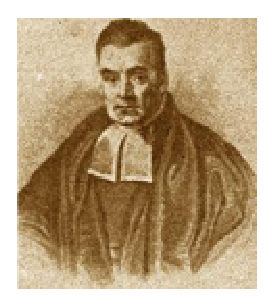
\includegraphics[height=3truecm]{figures/TBayes}
\end{columns}

\end{slide}\begin{slide}
\debut[Normal+improper]
If $x\sim\CN(\theta,1)$ and $\pi(\theta)=\varpi$, constant, 
the pseudo marginal distribution is 
$$
  m(x) =  \varpi \int^{+\infty }_{-\infty} {1 \over \sqrt{ 2\pi} }  
     \exp \left\{-(x-\theta)^2 /2 \right\} d\theta = \varpi
$$
and the posterior distribution of $\theta$ is
$${\Brown{
  \pi (\theta \mid x) = {1 \over \sqrt{ 2\pi}} 
     \exp \left\{ - {(x-\theta )^ 2 \over 2} \right\}  ,
}}$$
i.e., corresponds to ${\cal N}(x,1)$.
\emfarite{independent of $\varpi$}
\fin

\end{slide}\begin{slide}
\slidetitle{Meaningless as probability distribution}

\small\begin{flushright}\begin{quote}
The mistake is to think of them [the non-informative priors]\\
as representing ignorance\\
---Lindley, 1990---
\end{quote}\end{flushright}\normalsize

\pause
\debut Consider a $\theta\sim\CN(0,\tau^2)$ prior. Then
$$
  P^\pi\left( \theta \in [a,b] \right) \longrightarrow 0
$$
when ${\tau\to\infty}$ for any $(a,b)$
\fin

\end{slide}
\begin{slide}\slidetitle{Noninformative prior distributions}

\bigskip
\centerline{\Red{\fbox{\bf What if all we know is that we know ``nothing" ?!}}}

\pause
\bigskip
In the absence of prior information, prior distributions solely derived from the sample distribution \
$f(x|\theta)$

\pause\bigskip
\small\begin{flushright}\begin{quote}
Noninformative priors cannot be expected to represent exactly total ignorance
about the problem at hand, but should rather be taken as reference or 
default priors, upon which everyone could fall
back when the prior information is missing.\\
---Kass and Wasserman, 1996---
\end{quote}\end{flushright}\normalsize


\end{slide}\begin{slide}
\slidetitle{Laplace's prior}

Principle of {\it Insufficient Reason} (Laplace)
$$
\Theta = \{\theta_1,\cdots,\theta_p\}  \hspace{1cm}  \pi(\theta_i)=1/p
$$

\pause\smallskip
Extension to continuous spaces
{\Red{
$$
\pi(\theta) \propto 1
$$
}}
\emfarite{Lebesgue measure}

\end{slide}
\begin{slide}
\slidetitle{\Blue{\sf Who's Laplace?}}

\begin{block}{\BrickRed{{\bf Pierre Simon de Laplace (1749--1827)}}}
\begin{columns}\column{.55\textwidth}
French mathematician and astronomer born in Beaumont en Auge (Normandie)
who formalised mathematical astronomy in {\em M\'ecanique C\'eleste}. 
Survived the French revolution, the Napoleon Empire (as a comte!), and
the Bourbon restauration (as a marquis!!).

\column{.4\textwidth}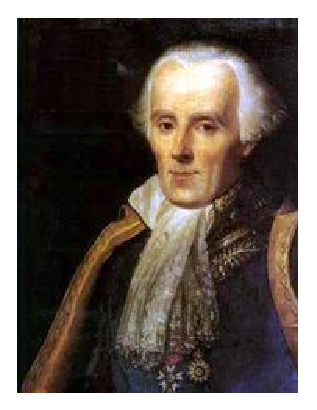
\includegraphics[height=3truecm]{figures/Laplace}
\end{columns}

\medskip
\pause
In {\em Essai Philosophique sur les Probabilit\'es}, Laplace set out a mathematical system of inductive 
reasoning based on probability, precursor to Bayesian Statistics. 
\end{block}

\end{slide}\begin{slide}
\slidetitle{Laplace's problem}

\begin{itemize}
\item  Lack of reparameterization invariance/coherence
{\Brown{
$$
\pi(\theta)\propto 1,\quad\text{and}\quad
\psi = e^{\theta}  \hspace{0.5cm}  \pi(\psi)={1\over\psi} \neq 1 \quad (!!)
$$
}}

\pause\item  Problems of properness
$$
{\Brown{
x\sim {\cal N}(\mu,\sigma^2),  \hspace{1cm}  \pi(\mu,\sigma)=1
}}
$$
$$
{\Brown{
\begin{array}{llll}
\space & \pi(\mu,\sigma|x) &\propto& e^{-(x-\mu)^2/2\sigma^2} 
\sigma^{-1} \\
\Rightarrow & \pi(\sigma|x) &\propto& 1 \qquad (!!!)
\end{array}
}}
$$
\end{itemize}

\end{slide}\begin{slide}
\slidetitle{Jeffreys' prior}

\begin{columns}\column{.55\textwidth}
Based on Fisher information
$$\BrickRed{
I^F (\theta) = \e_{\theta}\left[{\partial\log\ell\over\partial\theta^t}\;
              {\partial\log\ell\over\partial\theta}\right]
}$$
\column{.45\textwidth}
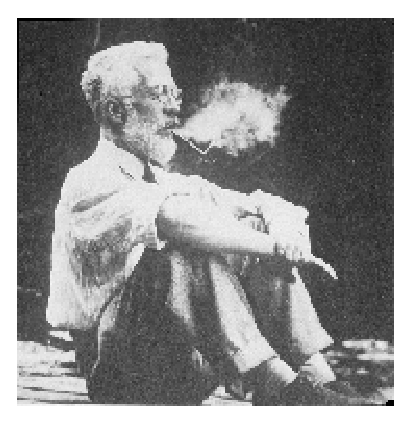
\includegraphics[height=3truecm]{figures/RonSmoke}\\
\small{\bf Ron Fisher (1890--1962)}\normalsize
\end{columns}

\pause
the Jeffreys prior distribution is 
{\Red{
$$
  \pi^J (\theta ) \propto |I^F (\theta)|^{1/2}
$$
}}

\end{slide}\begin{slide}
\slidetitle{\Blue{\sf Who's Jeffreys?}}

\begin{block}{{\BrickRed{{\bf Sir Harold Jeffreys (1891--1989) }}}}
\begin{columns}\column{.5\textwidth}
English mathematician, statistician, geophysicist, and astronomer. Founder of English Geophysics \&\
originator of the theory that the Earth core is liquid.

\pause
Formalised Bayesian methods for the analysis of geophysical data and ended up writing {\em Theory
of Probability}
\column{.4\textwidth}
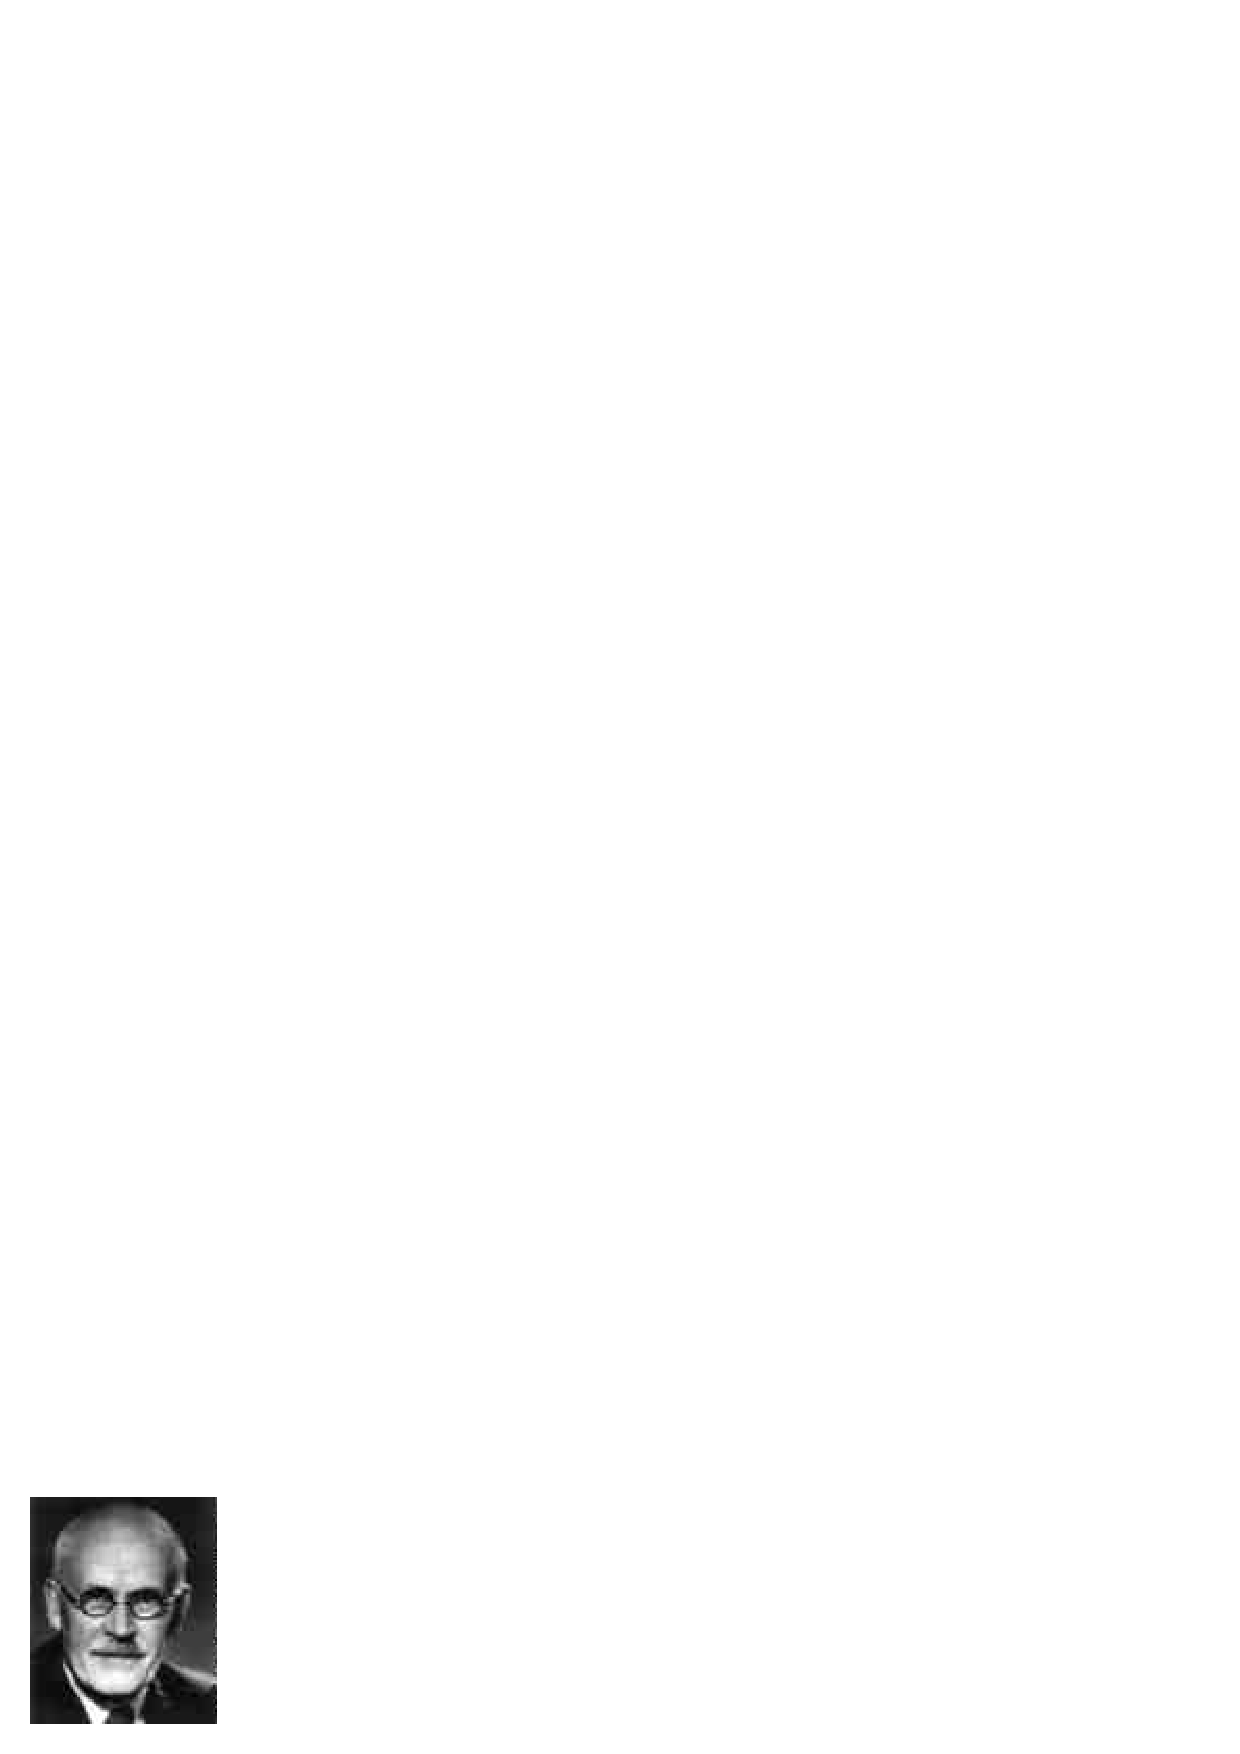
\includegraphics[height=3.5truecm]{figures/Jeffreys}
\end{columns}\end{block}

\end{slide}\begin{slide}
\slidetitle{Pros \&\ Cons}

\begin{itemize}    
\item  Relates to information theory
\pause
\item  Agrees with most invariant priors
\pause
\item  Parameterization invariant
\pause
\item  Suffers from dimensionality curse
\end{itemize}    

\end{slide}
\subsection{Bayesian estimation}
\begin{slide}
\slidetitle{Evaluating estimators}

Purpose of most inferential studies:
to provide the statistician/client with a
{\it decision} $d\in\CD$

\pause
Requires an evaluation criterion/{\sf loss function} for decisions and estimators
{\Red{$$
\Lrm(\theta,d)
$$}}

\pause\bigskip
{\RedOrange{\bf
There exists an axiomatic derivation
of the existence of a loss function.
}}
\rightline{\Brown{\sf [DeGroot, 1970]}}

%\end{slide}\begin{slide}
%\slidetitle{Bayesian \DT}

%Three spaces/factors:
%\begin{itemize}
%\item[(1)] On $\CX$, distribution for the observation,    $f(x|\theta)$;
%\item[(2)] On $\Theta$, prior distribution for the parameter,       $\pi(\theta)$;
%\item[(3)] On $\Theta\times\CD$, 
           %loss function associated with the decisions, $\Lrm(\theta,\delta)$;
%\end{itemize}

\end{slide}\begin{slide}
\slidetitle{Loss functions}

Decision procedure $\delta^\pi$ usually called
{\RedViolet{\sf estimator}}\\ (while its {\it value} $\delta^\pi(x)$
is called {\RedViolet{\sf estimate}} of $\theta$)

\pause\bigskip
Impossible to uniformly minimize  (in $d$)  the loss function
$$
\Lrm(\theta,d)
$$
when $\theta$ is unknown

%\end{slide}\begin{slide}
%\slidetitle{Frequentist Principle}

%Average loss (or {\RedViolet{\sf frequentist risk}})
%\begin{eqnarray*}
%R(\theta,\delta) & = & \BE_\theta \lbrack \Lrm (\theta
%,\delta(x))\rbrack \\
	%& = & \int_{\cal X} \Lrm(\theta,\delta(x))f(x|\theta) \,dx
%\end{eqnarray*}

%\medskip\pause
%{\BurntOrange{\bf Principle}} Select the best estimator based on the risk function

%\end{slide}\begin{slide}
%\slidetitle{Difficulties with frequentist paradigm}

%\begin{enumerate}
%\item Error averaged over the different values
%of $x$ proportionally to the density $f(x|\theta)$:
%not so appealing for a client, who wants
%optimal results for {\Red{\bf her}} data $x$!
%\pause\item Assumption of repeatability of experiments not always grounded.
%\pause\item $R(\theta, \delta)$ is a function of $\theta$: there is no
%total ordering on the set of procedures. 
%\end{enumerate}

\end{slide}\begin{slide}
\slidetitle{Bayesian estimation}
{\BurntOrange{\bf Principle}} Integrate over the space $\Theta$
to get the posterior expected loss
\begin{eqnarray*}
      & = & \BE^\pi[\Lrm(\theta,d)|x] \\
      & = & \int_{\Theta} \Lrm(\theta,d) \pi(\theta|x)\, d\theta,
\end{eqnarray*}
and minimise in $d$

\end{slide}\begin{slide}
\slidetitle{Bayes estimates}
{\Blue{
\begin{block}{Bayes estimator}
A {\Red{\em Bayes estimate}}\ associated with a prior distribution $\pi$ and a loss function $\Lrm$ is 
$$
  \arg\min_d \BE^\pi[\Lrm(\theta,d)|x] \,.
$$
\end{block}
}}

\end{slide}
%\subsubsection{Usual loss functions}\label{sec:2.5}
\begin{slide}
\slidetitle{The quadratic loss}

\begin{columns}\column{.6\textwidth}
Historically, first loss function (Legendre, Gauss, Laplace)
\[
	\Lrm (\theta ,d)  =  (\theta -d)^2
\]
\column{.4\textwidth}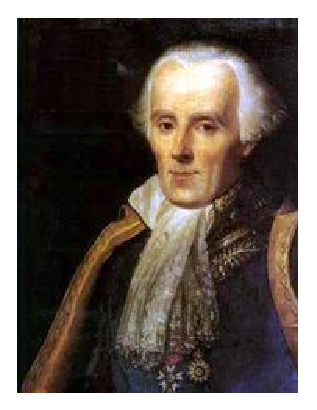
\includegraphics[height=3truecm]{figures/Laplace}
\end{columns}


%\end{slide}\begin{slide}
%\slidetitle{Proper loss}

\pause\smallskip {\RawSienna{
The Bayes estimate $\delta^\pi(x)$ associated with the prior $\pi$ and with the quadratic loss
is the posterior expectation
$$
\delta^\pi(x)  =  \BE^\pi[\theta|x]  = 
	{\int_\Theta \theta f(x|\theta)\pi(\theta) \,d\theta \over
		\int_\Theta f(x|\theta)\pi(\theta) \,d\theta} .
$$
}}

\end{slide}\begin{slide}
\slidetitle{The absolute error loss}

Alternatives to the quadratic loss:
\[
\Lrm(\theta,d)  =  \mid \theta-d\mid,
\]
or
\begin{eqnarray*}
\Lrm_{k_1,k_2} (\theta ,d)  =  \begin{cases} k_2(\theta -d) &
   \hbox{if }\theta  > d , \cr
			k_1(d-\theta )  & \hbox{otherwise.} \cr
			\end{cases}
\end{eqnarray*}

\pause
{\RawSienna{
Associated Bayes estimate is
$(k_2/(k_1+k_2))$ fractile of $\pi(\theta|x)$
}}

\end{slide}\begin{slide}
\slidetitle{MAP estimator}

With no loss function, consider using
the {\RedViolet{\sf maximum a posteriori (MAP) estimator}}
$$
\arg\max_\theta \ell(\theta|x)\pi(\theta)
$$

\smallskip\pause
%\end{slide}\begin{slide}
%\slidetitle{Motivations}
\begin{itemize}
\item Penalized likelihood estimator
\pause
\item Further appeal in restricted parameter spaces
\end{itemize}

\end{slide}\begin{slide}
\debut[Binomial probability]
Consider $x|\theta\sim{\cal B}(n,\theta)$. 

Possible priors:
$$
\pi^J (\theta) = {1 \over B(1/2,1/2)} \theta^{-1/2} (1-\theta)^{-1/2}\,,
$$
$$
\pi_1(\theta) = 1 \quad \hbox { and } \quad \pi_ 2(\theta) = \theta^{-1}(1-\theta)^{-1} \,.
$$
\pause
Corresponding MAP estimators:
\small
\begin{eqnarray*}
\delta^{\pi_J} (x) &=& \max \left({x-1/2 \over n - 1} , 0 \right) , \\
\delta^{\pi_1} (x) &=&  x / n , \\
\delta^{\pi_2} (x) &=& \max \left({x-1 \over n-2} , 0 \right) .
\end{eqnarray*}
\normalsize
\fin

\end{slide}\begin{slide}
\slidetitle{Not always appropriate}
\debut[Fixed MAP] Consider  
$$
f(x | \theta ) = {1 \over \pi}  \left[1+(x-\theta )^2 \right]^{-1},
$$
and $\pi(\theta)={1 \over 2} e^{-|\theta |}$.
\pause
Then the MAP estimate of $\theta$ is always
\[\Brown{
  \delta^\pi (x) = 0
}\]
\fin

\end{slide}
\subsection{Confidence regions}\begin{slide}
\slidetitle{Credible regions}

Natural confidence region: Highest posterior density (HPD) region
$$
C_\alpha^\pi =  \lbrace \theta;\pi(\theta |x)>k_\alpha\rbrace
$$
%\rightline{\Purple{\sf Highest posterior density (HPD) region}}

\pause
\begin{block}{Optimality}
\begin{columns}\column{.55\textwidth}
The HPD regions give the highest probabilities of containing $\theta$ for a given volume
\column{.4\textwidth}
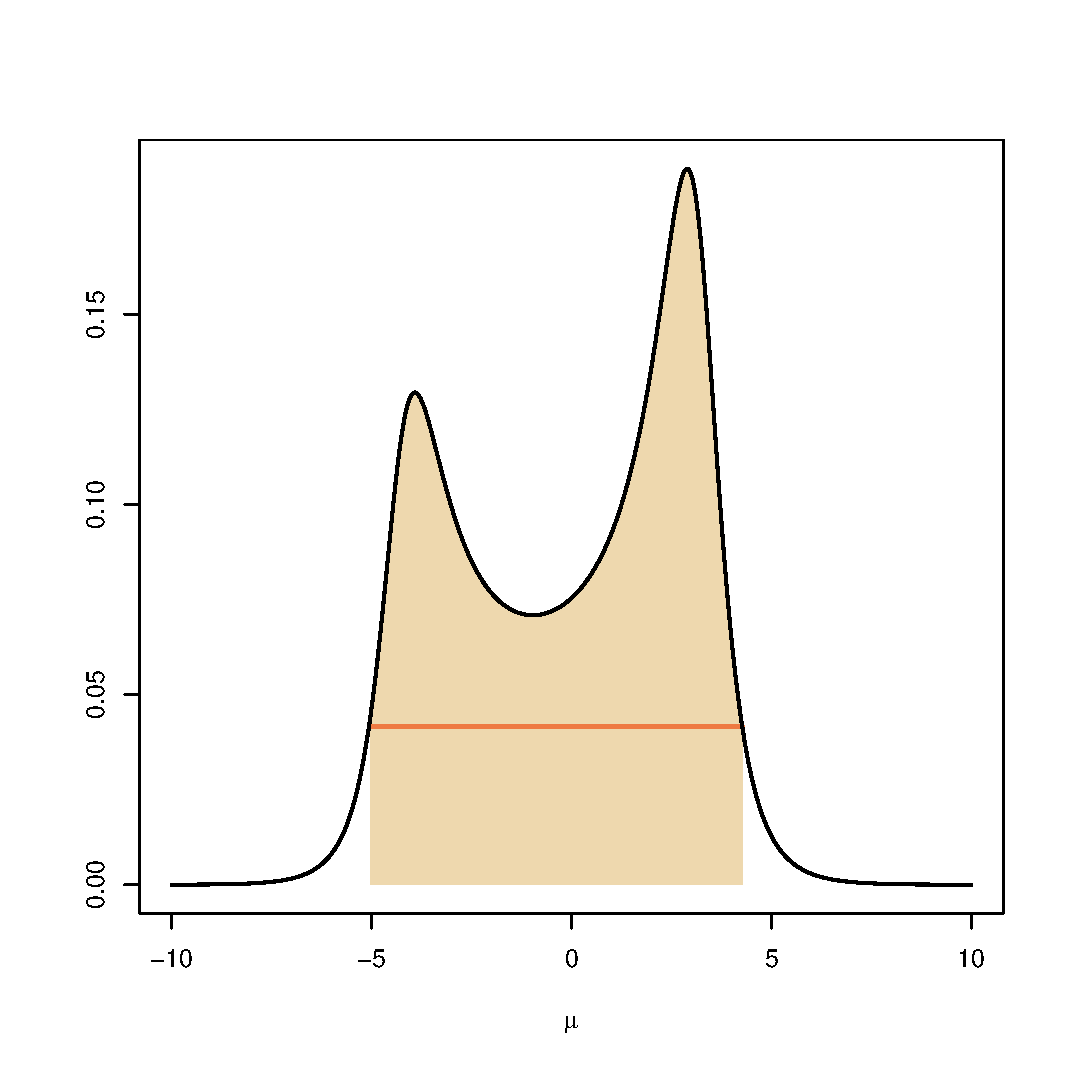
\includegraphics[width=4cm,height=4truecm]{figures/2cau}
\end{columns}
\end{block}

\end{slide}\begin{slide}
\debut If the posterior distribution of $\theta$ is 
${\cal N}(\mu(x),\allowbreak\omega^{-2})$ with $\omega^2=\tau^{-2}+\sigma^{-2}$ and 
$\mu(x)= \tau^2 x/(\tau^2+\sigma^2)$,
then
$$
C^\pi_\alpha  =  \left[\mu(x)-k_{\alpha} \omega^{-1}, \mu(x)+k_{\alpha} 
\omega^{ -1} \right],
$$
where $ k_\alpha $ is the $\alpha/2$-quantile of ${\cal N}(0,1)$. 

\pause
If $\tau$ goes to $+\infty$,
$$
C_\alpha^\pi =\left[x-k_{\alpha} \sigma , x+k_{\alpha} \sigma \right] ,
$$
the ``usual" (classical) confidence interval
\fin

\end{slide}
%\subsection{Normal model again}
\begin{slide}\slidetitle{Full normal}

Under [almost!] {\em Jeffreys prior} prior 
$$
\pi(\mu,\sigma^2)=1/\sigma^2,
$$
posterior distribution of $(\mu,\sigma)$
\small\begin{eqnarray*}
\mu|\sigma,{\bar x},s_x^2 & \sim & \CN\left({\bar x},{\sigma^2\over n}\right), \nonumber \\
\sigma^2|{\bar x},s_x^2   & \sim & {\cal IG}\left({n-1\over 2},{s_x^2\over 2}\right).
\end{eqnarray*}\normalsize

\smallskip\pause
Then
\begin{eqnarray*}\small
\pi(\mu|{\bar x},s_x^2)  & \propto & \int \omega^{1/2}\,\exp-\omega\frac{n({\bar x}-\mu)^2}{2}\,\omega^{(n-3)/2}\,\exp\{-\omega s_x^{2}/2\}\,\text{d}\omega \\
	                     & \propto & \left[ s_x^2 + n({\bar x}-\mu)^2 \right]^{-n/2}
\end{eqnarray*}\normalsize
\emfarite{$\mathcal{T}_{n-1}$ distribution}

\end{slide}\begin{slide}\slidetitle{Normal credible interval}

Derived credible interval on $\mu$
$$
[\bar x - t_{\alpha/2,n-1}s_x\big/\sqrt{n(n-1)},\bar x +t_{\alpha/2,n-1}s_x\big/\sqrt{n(n-1)}]
$$

\medskip\pause
\begin{block}{{\sf normaldata}}
Corresponding $95\%$ confidence region for $\mu$ 
$$
[-0.070,-0.013,]
$$ 
Since $0$ does not belong to this interval, reporting 
a significant decrease in the number of larcenies between 
1991 and 1995 is acceptable
\end{block}

\end{slide}
\subsection{Testing}\begin{slide}
%\subsubsection{The $0-1$ loss}
\slidetitle{Testing hypotheses}

Deciding about validity of assumptions or restrictions on
the parameter $\theta$ from the data, represented as
$$\BrickRed{
H_0:\theta \in\Theta_0 \quad\text{versus}\quad H_1:\theta \not\in\Theta_ 0
}$$

\pause
Binary outcome of the decision process: {\em accept} [coded by 1] or {\em reject\/} [coded by 0]
$$\BrickRed{
  \CD  =  \lbrace 0,1 \rbrace
}$$

\pause
Bayesian solution formally very close from a likelihood ratio test statistic, but
numerical values often strongly differ from classical solutions

\end{slide}\begin{slide}
\slidetitle{The $0-1$ loss}

Rudimentary loss function
$$
L (\theta ,d)  =  \begin{cases} 1-d & \hbox{if }\theta \in \Theta_0 \cr
			  d    &  \hbox{otherwise,} \cr \end{cases}
$$

Associated Bayes estimate
$$\RawSienna{
\delta^\pi(x) = \begin{cases} 1 &\hbox{if }P^\pi(\theta\in\Theta_0|x)
                        >\displaystyle{\frac{1}{2}},\cr
        0 & \hbox{otherwise.} \end{cases}
}$$

\pause
Intuitive structure

\end{slide}\begin{slide}
\slidetitle{Extension} 

Weighted $0-1$ (or $a_0-a_1$) loss
\begin{equation*}
\Lrm(\theta, d) = \begin{cases} 0 & \hbox{if } d=\BI_{\Theta_0}(\theta), \cr
           a_0 & \hbox{if }\theta\in\Theta_0\hbox{ and } d=0, \cr
           a_1 & \hbox{if }\theta\not\in\Theta_0\hbox{ and }d=1, \cr\end{cases}
\end{equation*}

\pause
\begin{block}{Associated Bayes estimator}
$$\RawSienna{
\delta^\pi(x) = \begin{cases} 1 &\hbox{if }P^\pi(\theta\in\Theta_0|x)
                        >\displaystyle{a_1\over a_0+a_1},\cr
	0 & \hbox{otherwise.} \end{cases}
}$$
\end{block}
\end{slide}\begin{slide}
\debut[Normal-normal] For $x\sim \CN(\theta,\sigma^2)$ 
and $\theta\sim\CN(\mu,\tau^2)$, $\pi(\theta|x)$ is 
$\CN(\mu(x),\omega^2)$ with
$$
\mu(x) = {\sigma^2\mu+\tau^2 x\over \sigma^2 +\tau^2} \quad \hbox{ and }
\quad \omega^2={\sigma^2\tau^2 \over \sigma^2+\tau^2}.
$$
\pause
To test $H_0:\,\theta<0$, we compute
\begin{eqnarray*}
P^\pi(\theta<0|x) &=& P^\pi\left({\theta-\mu(x)\over \omega} < 
			{-\mu(x)\over \omega} \right) \\
		&=& \Phi\left(-\mu(x)/ \omega \right). 
\end{eqnarray*}
\fin

\end{slide}\begin{slide}
\debut[Normal-normal (2)] If $z_{a_0,a_1}$ is the $a_1/(a_0+a_1)$ quantile, i.e., 
$$\Phi(z_{a_0,a_1})=a_1/(a_0+a_1)\,,$$ 
$H_0$ is accepted when
$$
  -\mu(x) > z_{a_0,a_1} \omega,
$$
the upper acceptance bound then being 
$$\BrickRed{
x \le - {\sigma^2 \over \tau^2} \mu - (1+{\sigma^2\over \tau^2}) 
\omega z_{a_0,a_1}.
}$$
\fin

\end{slide}\begin{slide}
\slidetitle{Bayes factor}
Bayesian testing procedure depends on $P^\pi (\theta \in \Theta_0|x)$ 
or alternatively on the \Blue{{\bf Bayes factor}}
$$
\BrickRed{
B^\pi_{10} = \frac{\left\{ P^\pi(\theta \in \Theta_1|x) / P^\pi(\theta \in \Theta_0|x) \right\} 
}{ \left\{ P^\pi(\theta \in \Theta_1)/ P^\pi(\theta \in \Theta_0) \right\} }
}$$
in the absence of loss function parameters $a_0$ and $a_1$

\end{slide}\begin{slide}
\slidetitle{Associated reparameterisations}

Corresponding models ${\cal M}_1$ vs. ${\cal M}_0$ compared via
$$
B_{10}^\pi = \displaystyle{ {P^\pi ({\cal M}_1|x) \over P^\pi ({\cal M}_0|x)} \bigg/
{P^\pi ({\cal M}_1) \over P^\pi  ({\cal M}_0)} } 
$$

\pause
If we rewrite the prior as 
\centerline{$\pi(\theta) = \hbox{Pr}(\theta\in\Theta_1)\times\pi_1(\theta) +
		\hbox{Pr}(\theta\in\Theta_0)\times\pi_0(\theta)$}
then
$$
B_{10}^\pi = { \displaystyle{\int f(x|\theta_1) \pi_1(\theta_1) \text{d}\theta_1} }\bigg/{
\displaystyle{\int f(x|\theta_0) \pi_0(\theta_0) \text{d}\theta_0} } = m_1(x)/m_0(x)
$$
\emfarite{{\bf Akin to likelihood ratio}}

\end{slide}\begin{slide}
\slidetitle{Jeffreys' scale}
\begin{columns}\column{.65\textwidth}
\begin{enumerate}
   \item if $\log_{10} (B^\pi_{10})$ varies between $0$ and $0.5$,
           the evidence against $H_0$ is {\it poor},
   \item if it is between $0.5$ and $1$, it is is {\it substantial},
   \item if it is between $1$ and $2$, it is {\it strong}, and
   \item if it is above $2$ it is {\it decisive}.
\end{enumerate}
\column{.3\textwidth}
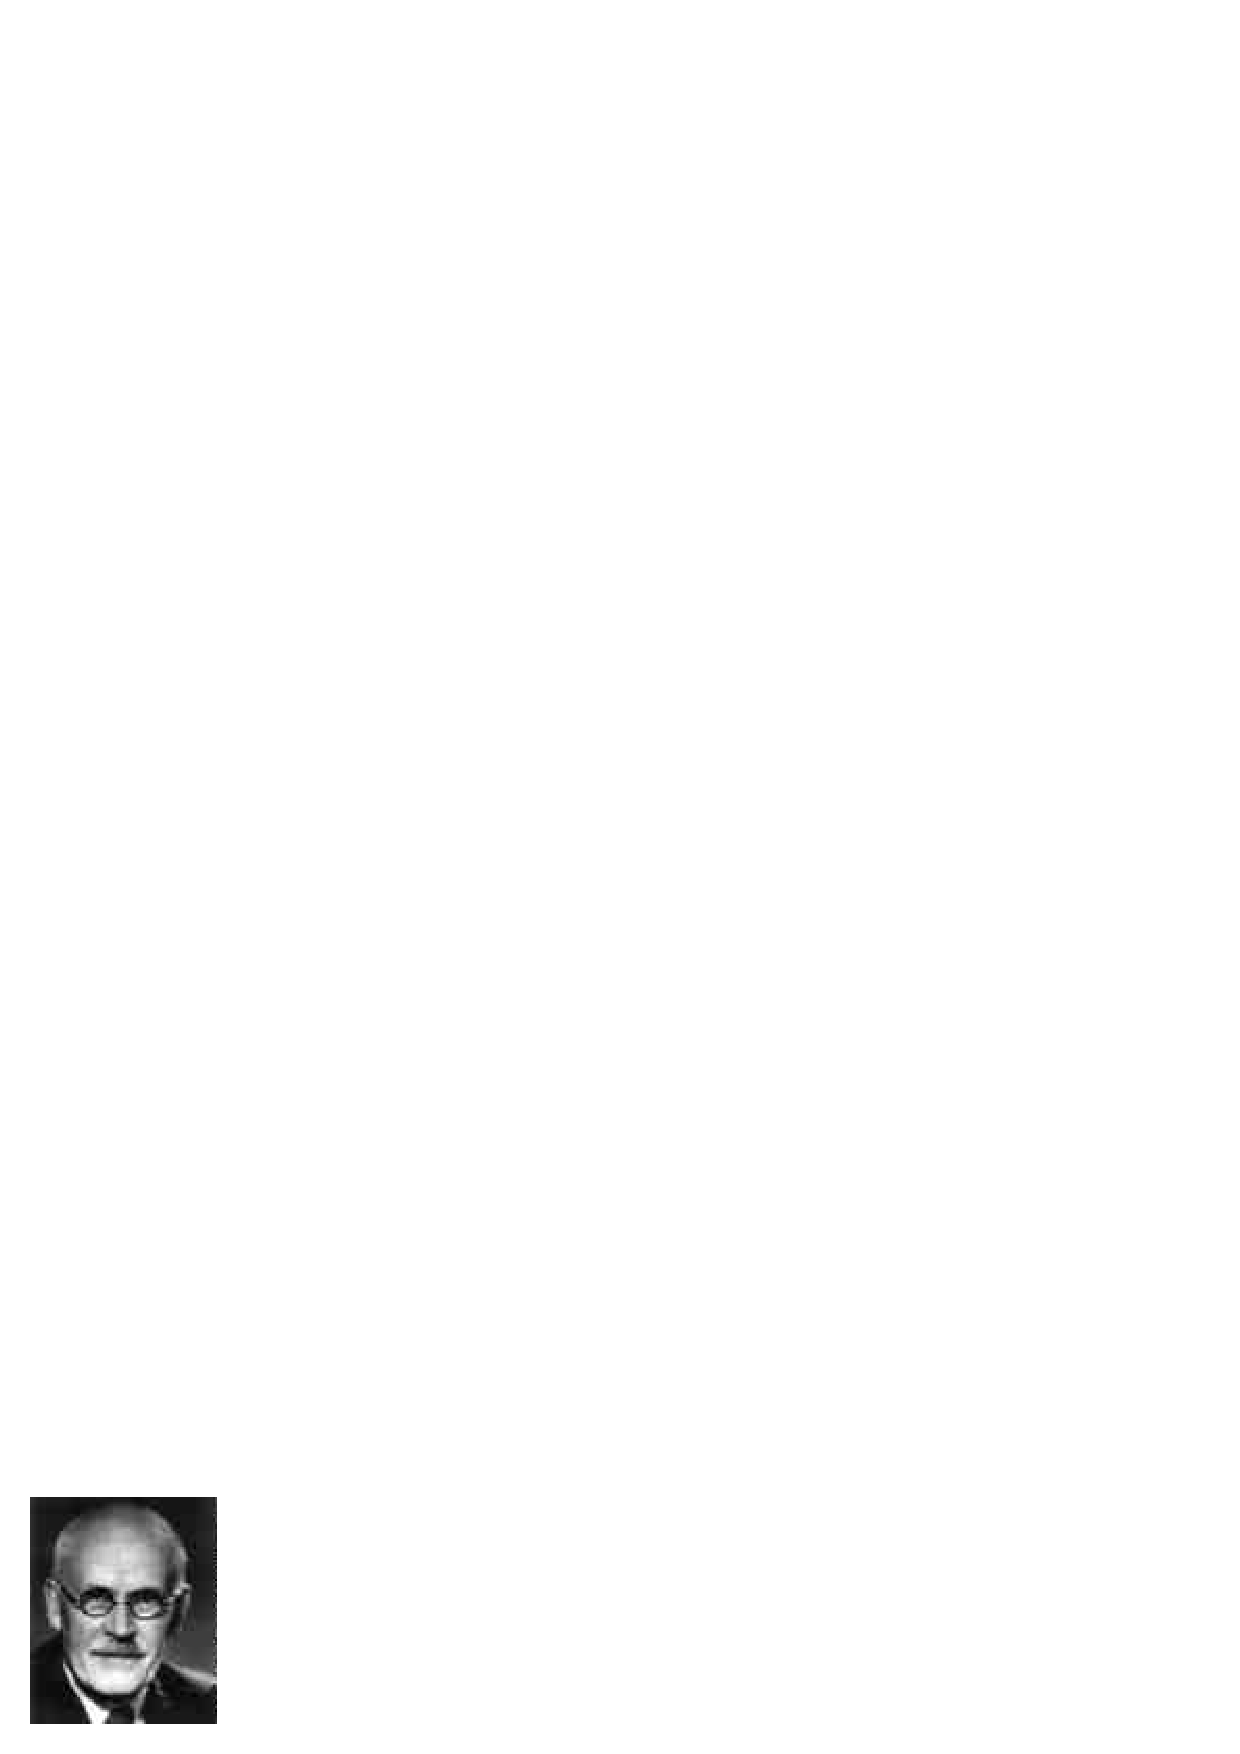
\includegraphics[height=3truecm]{figures/Jeffreys}
\end{columns}

\end{slide}\begin{slide}
\slidetitle{Point null difficulties}

If $\pi$ absolutely continuous, 
$$P^\pi(\theta=\theta_0)=0\ldots$$

\pause
\vglue 1truecm
\centerline{\BurntOrange{\fbox{{\bf How can we test $H_0:\theta=\theta_0$?!}}}}

\end{slide}\begin{slide}
\slidetitle{New prior for new hypothesis}

Testing point null difficulties requires a modification of the prior distribution
so that 
$$\Brown{
\pi(\Theta_0)>0 \quad\hbox{and}\quad \pi(\Theta_1)>0
}$$
(hidden information) or
$$\Brown{
\pi(\theta) = P^\pi (\theta\in\Theta_0)\times\pi_0(\theta) +
                P^\pi (\theta\in\Theta_1)\times\pi_1(\theta)
}$$


\pause
\emfarite{E.g., when $\Theta_0=\{\theta_0\}$, $\pi_0$ is Dirac mass at $\theta_0$}

\end{slide}\begin{slide}
\slidetitle{Posteriors with Dirac masses}

If $H_0: \ \theta=\theta_0$ $(=\Theta_1)$, 
$$
\rho = P^\pi (\theta=\theta_0) \quad\hbox{and}\quad
\pi(\theta) = \rho \BI_{\theta_0}(\theta)+ (1-\rho) \pi_1(\theta)
$$
then
\begin{align*}
\pi(\Theta_0|x) &= {f(x|\theta_0)\rho \over 
		\int f(x|\theta)\pi(\theta)\,d\theta} \\
 &= \BrickRed{{f(x|\theta_0)\rho \over f(x|\theta_0)\rho + (1-\rho) m_1(x)}}
\end{align*}
with
$$
m_1(x)=\int_{\Theta_1} f(x|\theta)\pi_1(\theta)\,d\theta.
$$

\end{slide}\begin{slide}
\debut[Normal-normal] For $x\sim \CN(\theta,\sigma^2)$ and $\theta\sim\CN(0,\tau^2)$,
to test of $H_0:\theta=0$ requires a modification of the prior, with
$$\RawSienna{
\pi_1(\theta) \propto e^{-\theta^2/2\tau^2} \mathbb{I}_{\theta\ne 0}
}$$
and $\pi_0(\theta)$ the Dirac mass in $0$

\pause
Then
\begin{eqnarray*}
{m_1(x)\over f(x|0)} &=&  {\sigma\over \sqrt{\sigma^2+\tau^2}}
	{e^{-x^2/2(\sigma^2+\tau^2)} \over e^{-x^2/2\sigma^2}} \\
      &=&  \sqrt{{\sigma^2\over\sigma^2+\tau^2}} \exp\left\{
	   {\tau^2x^2\over 2\sigma^2(\sigma^2+\tau^2)} \right\}, 
\end{eqnarray*}
\fin

\end{slide}\begin{slide}
\debut[cont'd]
and
$$
\pi(\theta=0|x) = \left[ 1+{1-\rho\over \rho} \sqrt{{\sigma^2\over
\sigma^2+\tau^2}} \exp\left({\tau^2x^2\over 2\sigma^2(\sigma^2+\tau^2)}\right)
\right]^{-1}.
$$

For $z=x/\sigma$ and $\rho=1/2$:
 
\centerline{
\MidnightBlue{\begin{tabular}{|c|c|c|c|c|}
\hline
$ z $ & $ 0$ & $ 0.68 $ & $ 1.28$ & $ 1.96 $ \cr
\hline
$ \pi(\theta=0| z,\tau=\sigma) $ & $ 0.586$ & $ 0.557 $ & $ 0.484$ & $ 0.351 $ \cr
$ \pi(\theta =0|z,\tau=3.3\sigma) $ & $ 0.768$ & $ 0.729 $ & $ 0.612$ & $ 0.366 $ \cr
\hline
\end{tabular}}}
\fin

\end{slide}\begin{slide}
\slidetitle{Banning improper priors}

Impossibility of using improper priors for testing!

\medskip\pause
\Brown{{\bf Reason:}} When using the representation
$$
\pi(\theta) = P^\pi (\theta\in\Theta_1)\times\pi_1(\theta) +
              P^\pi (\theta\in\Theta_0)\times\pi_0(\theta)
$$
$\pi_1$ and $\pi_0$ must be normalised

\end{slide}\begin{slide}
\debut[Normal point null] When $x\sim \CN(\theta,1)$ and $H_0:\ \theta=0$, for
the improper prior $\pi(\theta)=\Red{{\mathbf 1}}$, the prior is transformed as
$$
\pi(\theta)  = {1\over 2} \BI_{0}(\theta) + {1\over 2} \cdot \Red{{\mathbf \BI_{\theta\ne 0}}},
$$
and
\begin{eqnarray*}
\pi(\theta=0|x) &=& {e^{-x^2/2}\over e^{-x^2/2}+\int_{-\infty}^{+\infty}
   e^{-(x-\theta)^2/2} \,d\theta} \\
&=&  {1 \over 1+\sqrt{2\pi} e^{x^2/2} }.
\end{eqnarray*}
\fin

\end{slide}\begin{slide}
\debut[Normal point null (2)] 
\RawSienna{{\bf Consequence:}} 
$H_0$ is bounded from above by 
$$
\pi(\theta=0|x) \le 1/(1+\sqrt{2\pi})=0.285
$$
\MidnightBlue{\centerline{
\begin{tabular}{|c|c|c|c|c|c|}
\hline
$x $ & $ 0.0$ & $ 1.0 $ & $ 1.65$ & $ 1.96 $ & $ 2.58 $ \cr
\hline
$ \pi(\theta=0| x)$ & $0.285 $ &$0.195$ & $0.089 $ & $0.055$ & $0.014$ \cr
\hline
\end{tabular}
}}
\fin

\medskip
\RawSienna{{\bf Regular tests:}}
Agreement with the classical $p$-value (but...)

\end{slide}\begin{slide}
\debut[Normal one-sided] For $x\sim\CN(\theta,1)$, $\pi(\theta)=1$, 
and $H_0:\ \theta\le 0$ to test versus $H_1: \theta>0$
$$
\pi(\theta\le 0|x) =  {1\over \sqrt{2\pi} } \int_{-\infty}^0 
	e^{-(x-\theta)^2/2} \,d\theta =  \Phi(-x). 
$$
The generalized Bayes answer is also the {\it $p$-value}
\fin

\pause\medskip
\begin{block}{{\sf normaldata}}
If $\pi(\mu,\sigma^2)=1/\sigma^2$, 
$$
\pi(\mu\ge 0|x) = 0.0021
$$
since $\mu|x\sim\mathscr{T}_{89}(-0.0144,0.000206)$.
\end{block}

\end{slide}\begin{slide}
\slidetitle{Jeffreys--Lindley paradox}

\BurntOrange{{\sffamily\bfseries Limiting arguments not valid in testing settings:}}
Under a conjugate prior
$$
\pi(\theta=0|x) = \left\{ 1+{1-\rho\over \rho} 
	\sqrt{{\sigma^2\over \sigma^2+\tau^2}} \exp
  \left[{\tau^2x^2\over 2\sigma^2(\sigma^2+\tau^2)}\right] \right\}^{-1} ,
$$
which converges to \BrickRed{$1$} when $\tau$ goes to $+\infty$, 
\Red{{\bf for every $x$}}

\medskip\pause
Difference with the ``noninformative'' answer 
$$
[1+\sqrt{2\pi}\exp(x^2/2)]^{-1}
$$
\emfarite{\BrickRed{{\Large $\lightning$} Invalid answer}}

\end{slide}\begin{slide}
\slidetitle{Normalisation difficulties}
If $g_0$ and $g_1$ are $\sigma$-finite measures 
on the subspaces $\Theta_0$ and $\Theta_1$, the choice of the normalizing constants 
influences the Bayes factor: 

\BurntOrange{{\bf If $g_i$ replaced by $c_ig_i$ $(i=0,1)$, 
Bayes factor multiplied by \Red{$c_0/c_1$}}}

\pause
\debut If the Jeffreys prior is uniform and $g_0=c_0$, $g_1=c_1$, 
\small
\begin{eqnarray*}
\pi(\theta\in\Theta_0|x) &=& {\rho c_0\int_{\Theta_0} f(x|\theta)\,d\theta
	    \over \rho c_0\int_{\Theta_0} f(x|\theta)\,d\theta +
	   (1-\rho)c_1\int_{\Theta_1} f(x|\theta)\,d\theta }\\
&=& {\rho \int_{\Theta_0} f(x|\theta)\,d\theta
            \over \rho \int_{\Theta_0} f(x|\theta)\,d\theta +
           (1-\rho)\Red{\mathbf{[c_1/c_0]}}\int_{\Theta_1} f(x|\theta)\,d\theta }
\end{eqnarray*}
\normalsize
\fin

\end{slide}
\subsection{Monte Carlo integration}\begin{slide}
\slidetitle{Monte Carlo integration}

Generic problem of evaluating an integral
\begin{displaymath}\Brown{
    {\mathfrak{I}} = \BE_f[h(X)] = \int_{\CX} \; h(x) \; f(x) \; dx \;
}\end{displaymath}
where $\CX$ is uni- or multidimensional, $f$ is a closed form, partly closed form, or implicit density,
and $h$ is a function

\end{slide}\begin{slide}
\slidetitle{Monte Carlo Principle}
Use a sample $(x_1,\ldots,x_{m})$  from the density $f$ 
to approximate the integral ${\mathfrak{I}}$ by the empirical average
$$
  {\overline{h}}_{m} = {1\over m} \; \sum_{j=1}^{m} \; h(x_{j})
$$

\medskip\pause
Convergence of the average 
$$
  {\overline{h}}_{m}  \longrightarrow \BE_f[h(X)]
$$
by the {\Blue{\bf Strong Law of Large Numbers}}

\end{slide}\begin{slide}
\slidetitle{Bayes factor approximation}

For the normal case 
\begin{eqnarray*}
x_1,\ldots,x_n&\sim&\mathscr{N}(\mu+\xi,\sigma^2)\\
y_1,\ldots,y_n&\sim&\mathscr{N}(\mu-\xi,\sigma^2)\\ 
\text{and} && H_0:\xi=0
\end{eqnarray*}
under prior 
$$
\pi(\mu,\sigma^2)=1/\sigma^2 \quad\text{ and }\quad \xi\sim\mathscr{N}(0,1)
$$
\small
$$
B^\pi_{01} = \frac{ \left[ (\bar x-\bar y)^2+S^2 \right]^{-n+1/2} }{
\int\,\left[ (2\xi-\bar x-\bar y)^2+S^2 \right]^{-n+1/2} \,e^{-\xi^2/2}\,\hbox{d}\xi/\sqrt{2\pi}}
$$
\normalsize

\end{slide}\begin{slide}
\slidetitle{Example}
\begin{block}{{\sf CMBdata}}
Simulate $\xi_1,\ldots,\xi_{1000}\sim\mathscr{N}(0,1)$ and approximate $B^\pi_{01}$ with
\small
$$
{\widehat{B^\pi_{01}}} = \frac{ \left[ (\bar x-\bar y)^2+S^2 \right]^{-n+1/2} }{
\frac{1}{1000}\,\sum_{i=1}^{1000} \left[ (2\xi_i-\bar x-\bar y)^2+S^2 \right]^{-n+1/2} } = 89.9
$$
\normalsize
when $\bar x = 0.0888\,,\quad \bar y = 0.1078\,,\quad S^2 = 0.00875$
\end{block}

\end{slide}\begin{slide}
\slidetitle{Precision evaluation}
Estimate the variance with
$$
  v_m =  {1\over m} \frac{1}{m-1} \sum_{j=1}^{m} \; [h(x_{j})-{\overline{h}}_{m}]^2,
$$
and for $m$ large,
$$ 
  \left\{ \overline{h}_m - \BE_f[h(X)] \right\}   / \sqrt{v_m} \approx \CN(0,1).
$$

\medskip\pause
\begin{block}{\Brown{\bf Note}} 
\begin{columns}
\column{.5\textwidth}
Construction of a convergence test
and of confidence bounds on the approximation of $\BE_f[h(X)]$
\column{.4\textwidth}
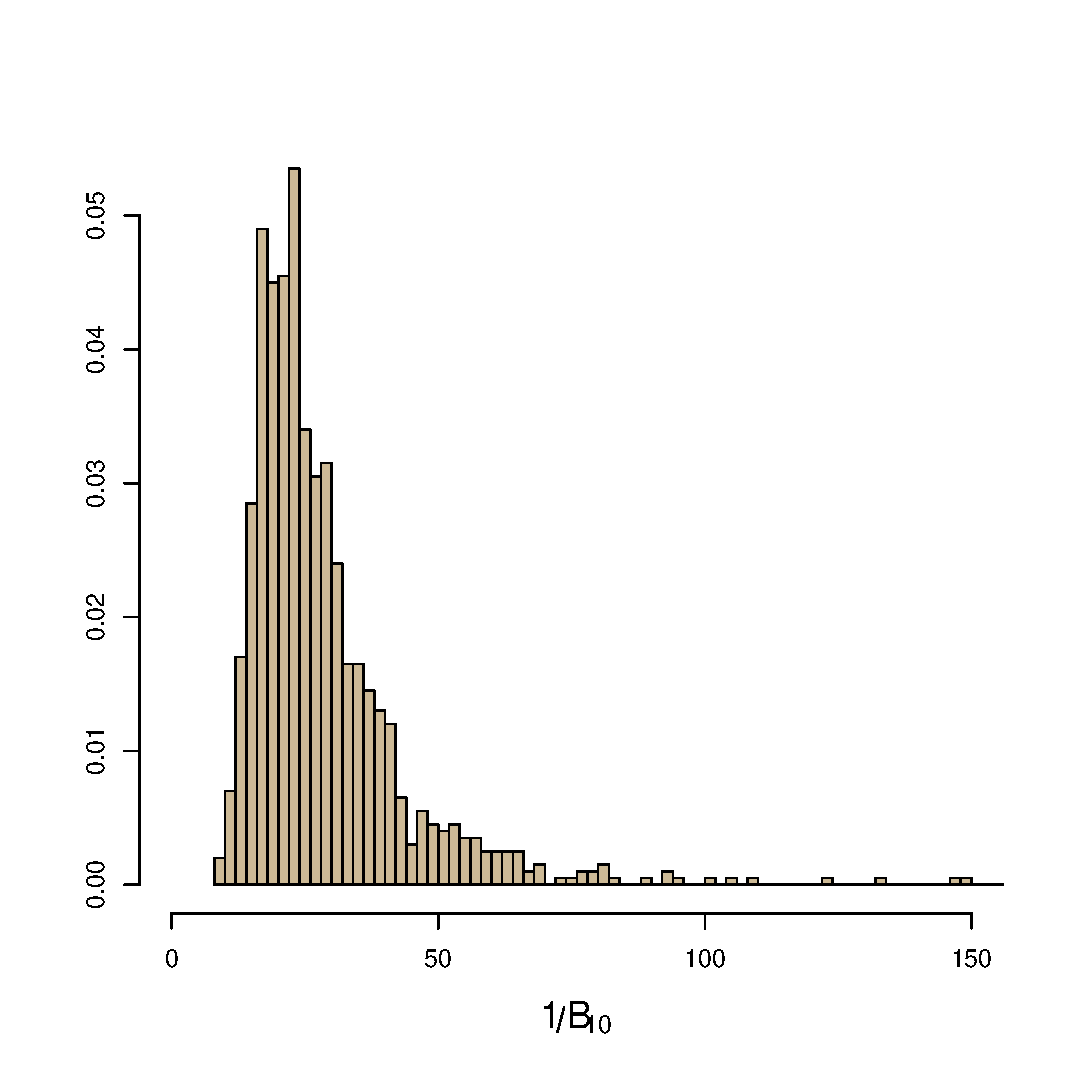
\includegraphics[height=3truecm]{figures/compbf}
\end{columns}
\end{block}

\end{slide}\begin{slide}
\debut[Cauchy-normal]
For estimating a normal mean, a 
{\it robust} prior is a Cauchy prior
$$
  x \sim \CN (\theta,1), \quad \theta \sim {\cal C}(0,1).
$$

Under squared error loss, posterior mean
$$
\delta^\pi(x)=\frac{\displaystyle{ \int_{-\infty}^{\infty} 
\frac{\theta}{1+\theta^2}} 
e^{-(x-\theta)^2/2} d\theta}{\displaystyle{\int_{-\infty}^{\infty} 
\frac{1}{1+\theta^2}} e^{-(x-\theta)^2/2} d\theta}
$$
\fin

\end{slide}\begin{slide}
\debut[Cauchy-normal (2)]
Form of $\delta^\pi$ suggests simulating iid variables 
$\theta_1, \cdots, \theta_m \sim \CN (x,1)$ and calculate
\begin{columns}\column{.48\textwidth}
\begin{displaymath}
 \hat{\delta}^\pi_m(x)=\frac{\sum_{i=1}^m 
\displaystyle{\frac{\theta_i}{1+\theta_i^2}}}{\sum_{i=1}^m 
\displaystyle{\frac{1}{1+\theta_i^2}}}  \;.
\end{displaymath}

\pause
LLN implies
$$\hat{\delta}^\pi_m(x) \longrightarrow 
\delta^\pi(x)\mbox{ as } m \longrightarrow \infty.$$ 
\column{.45\textwidth}
\includegraphics[height=\textwidth,width=5cm,angle=270]{figures/rangeofco.ps}
\end{columns}\fin

\end{slide}\begin{slide}
%\subsubsection{Importance Sampling}\label{sec:imosa}
\slidetitle{Importance sampling}

Simulation from $f$ (the true density) is not necessarily {\Red{\bf optimal}}

\medskip\pause
Alternative to direct sampling from $f$ is {\Emerald{\bf importance sampling}},
based on the alternative representation 
$$\Brown{
\BE_f[h(x)]  = \int_{\cal{X}} \; \left[ h(x) \; {f(x)\over g(x)} \right]\; g(x) \; dx
= \BE_g\left[ h(x)\frac{f(x)}{g(x)}\right]
}$$
which allows us to use \RawSienna{{\bf other}} distributions than $f$

\end{slide}\begin{slide}
\slidetitle{Importance sampling (cont'd)}
\begin{block}{Importance sampling algorithm}
Evaluation of
$$
  \BE_f[h(x)] = \int_{\CX} \; h(x) \; f(x) \; dx
$$
by 
{\sf \begin{enumerate}
\item Generate a sample $x_1,\ldots,x_m$ from a distribution $g$
\item Use the approximation
$$
 {1\over m}\; \sum_{j=1}^m\; {f(x_j)\over g(x_j)}\; h(x_j)
$$
\end{enumerate}
}\end{block}

\end{slide}\begin{slide}
\slidetitle{Justification}

Convergence of the estimator
$$
{1\over m}\; \sum_{j=1}^m\; {f(x_j)\over g(x_j)}\;h(x_j)
\longrightarrow  \BE_f[h(x)]
$$

\begin{enumerate}
\item converges for any choice
of the distribution $g$ as long as $\mathrm{ supp}(g) \supset \mathrm{ supp}(f)$

\pause
\item Instrumental distribution 
$g$ chosen from distributions easy to simulate

\pause
\item Same sample (generated from $g$) 
can be used repeatedly, not only for different functions 
$h$, but also for different densities $f$
\end{enumerate}

\end{slide}\begin{slide}
\slidetitle{Choice of importance function}
$g$ can be any density but some choices better than others

\begin{enumerate}
\item Finite variance only when 
$$
\BE_f \left[ h^2(x)  \frac{f(x)}{g(x)} \right] = \int_{\cal X}\; h^2(x)\; 
\frac{f^2(x)}{g(x)} \; dx < \infty \; .  
$$

\pause
\item Instrumental distributions with tails
lighter than those of $f$ (that is, with $\sup f/g = \infty$)
not appropriate, because weights $f(x_j)/g(x_j)$ vary widely,
giving too much importance to a few values $x_j$.

\pause
\item If $\sup f/g = M < \infty$, the accept-reject algorithm
can be used as well to simulate $f$ directly.

\pause
\item IS suffers from curse of dimensionality
\end{enumerate}


\end{slide}\begin{slide}
\debut[Cauchy target]
Case of Cauchy distribution $\mathcal{C}(0,1)$ when importance function is 
Gaussian $\mathscr{N}(0,1)$. 
\begin{columns}\column{.5\textwidth}
Density ratio 
$$
\frac{p^\star(x)}{p_0(x)}
= \sqrt{2\pi}\,\frac{\exp x^2/2}{\pi\,(1+x^2)}
$$
very badly behaved: e.g.,
$$
\int_{-\infty}^{\infty} \varrho(x)^2 p_0(x) dx = \infty
$$
\column{.45\textwidth}
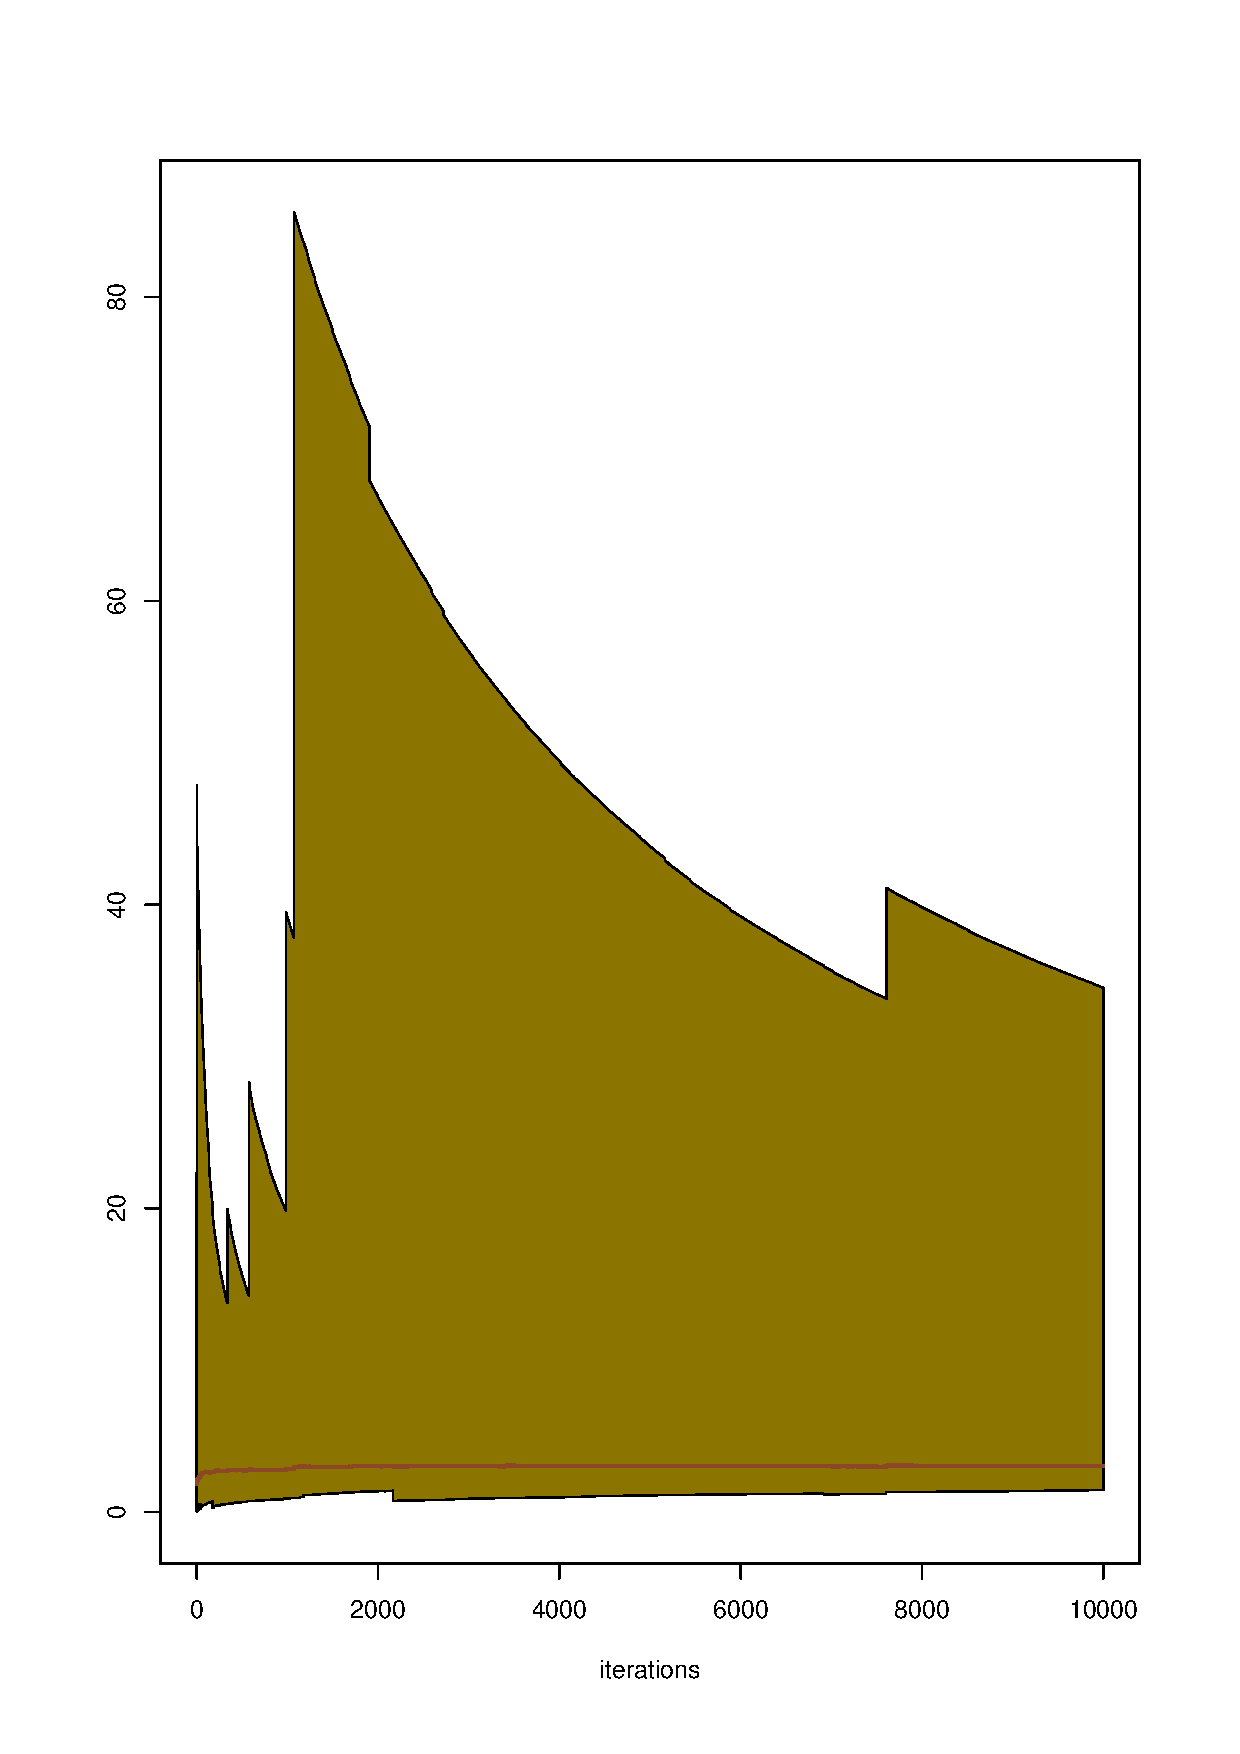
\includegraphics[height=3.5truecm,width=.9\textwidth]{figures/impinf}
\end{columns}

Poor performances of the
associated importance sampling estimator 
\fin

\end{slide}
\begin{slide}
\slidetitle{Practical alternative}
\begin{displaymath}
\sum_{j=1}^m \; h(x_{j}) \; f(x_{j}) / g(x_{j}) \bigg/
\sum_{j=1}^m \; f(x_{j}) / g(x_{j})
\end{displaymath}
where $f$ and $g$ are known up to constants.

\begin{enumerate}
\item Also converges to ${\mathfrak{I}}$ by the Strong Law of Large Numbers.
\item Biased, but the bias is quite small:
may beat the unbiased estimator in squared error loss.
\end{enumerate}  

\end{slide}\begin{slide}
\debut[Student's $t$ distribution]
$x \sim {\cal{T}}(\nu,\theta,\sigma^2)$, with density
$$
f_\nu(x) = {\Gamma((\nu+1)/2)\over \sigma \sqrt{\nu\pi} \; \Gamma(\nu/2)}
\left(1+{(x - \theta)^2\over \nu \sigma^2}\right)^{-(\nu+1)/2} \;. 
$$

Without loss of generality, take $\theta = 0$, $\sigma = 1$.

\pause
Integral of interest
$$
\mathfrak{I} = \int \sqrt{\left|{x\over 1-x}\right|} \,f_\nu(x) \,\hbox{d}x
$$
\fin

\end{slide}\begin{slide}
\debut[Student's $t$ distribution (2)]
\begin{columns}\column{.45\textwidth}
Choices of h:
\begin{enumerate}
\item Student \ \Brown{${\mathcal{T}}(\nu,0,1)$}  
\item Cauchy \ \Brown{${\mathcal{C}}(0,1)$}       
\item Normal \ \Brown{$\mathscr{N}(0,\nu/(\nu-2))$}   
\end{enumerate}

{\bf Note:} The ratio
$$\Red{
{f^2(x) \over h(x) } \propto
{e^{x^2(\nu-2)/2\nu}\over [1 + x^2/\nu]^{(\nu+1)}}
}$$
does not have a finite integral
\column{.5\textwidth}
\includegraphics[width=5cm,height=\textwidth,angle=270]{figures/student.range.eps} 
\end{columns}
\fin

\end{slide}\begin{slide}
\slidetitle{Explanation}
\debut[Student's $t$ distribution (3)]
Phenomenon due to the fact that $h$ has a singularity at $x=1$:
$$
\int \frac{|x|}{|1-x|} f_\nu(x) \,\hbox{d}x = \infty
$$

\pause
\Sepia{{\bf Consequence:} the three estimators have infinite variance}
\fin

\end{slide}\begin{slide}
\slidetitle{Alternative} 
\debut[Student's $t$ distribution (4)]
Choose a better behaved $h$: \pause
folded Gamma distribution, $x$ symmetric around $1$ with
\begin{columns}\column{.55\textwidth}
$$
|x-1| \sim\mathcal{G}a(\alpha,1)
$$ 
Then  $h_1(x)f^2(x)/h(x)$ proportional to
$$
\sqrt{x}\,f^2(x)\,|1-x|^{1-\alpha-1}\,\exp|1-x|
$$
integrable around $x=1$ when $\alpha<1$.
\column{.42\textwidth}
\includegraphics[width=4cm,height=\textwidth,angle=270]{figures/student.best.eps}
\end{columns}
\fin

\end{slide}\begin{slide}
\slidetitle{Choice of importance function (termin'd)}
{\BurntOrange{\fbox{\bf The importance function may be $\pi$}}}

\medskip\pause
\begin{itemize}
       \item  often inefficient if data informative
       \item  impossible if $\pi$ is improper
\end{itemize}

\pause\medskip
{\BurntOrange{\fbox{\bf Defensive sampling:}}}
$$
h(\theta) = \rho \pi(\theta) + (1-\rho) \pi(\theta|x) \qquad \rho\ll 1
$$
\end{slide}\begin{slide}
\debut[Cauchy/Normal] \ Consider
$$
  	x_1,\ldots,x_n \sim \CC(\theta,1)
\qquad \text{and} \qquad
	\theta\sim\CN(\mu,\sigma^2),
$$
with known \hypa s $\mu$ and $\sigma^2$.

\pause
Since $\pi(\theta)$ is normal $\CN(\mu, \sigma^2)$, possible 
to simulate a normal sample $\theta_1,\ldots,\allowbreak\theta_M$ 
and to approximate the Bayes estimator by
\[
\hat\delta^\pi(x_1,\ldots,x_n) =
{\sum_{t=1}^M \theta_t \prod_{i=1}^n [1+(x_i-\theta_t)^2]^{-1} \over 
\sum_{t=1}^M \prod_{i=1}^n [1+(x_i-\theta_t)^2]^{-1}}.
\]
\fin

\end{slide}\begin{slide}
\debut[Cauchy/Normal (2)]

Poor when the $x_i$'s are all far from $\mu$

\centerline{\includegraphics[height=10cm,angle=270,width=5cm]{figures/fig622.ps}}
$90\%$ range of variation 
for $n=10$ observations from $\CC (0,1)$ distribution and $M=1000$
simulations of $\theta$ as $\mu$ varies
\fin

\end{slide}\begin{slide}
\slidetitle{Bridge sampling}
Bayes factor
$$
B^\pi_{12} = { \displaystyle{\int f_1(x|\theta_1) \pi_1(\theta_1) d\theta_1} \over
\displaystyle{\int f_2(x|\theta_2) \pi_2(\theta_2) d\theta_2} }
$$

\pause
If
$$
\begin{array}{lll}
\pi_1(\theta_1|x) &\propto& {\tilde\pi}_1(\theta_1|x) \\
\pi_2(\theta_2|x) &\propto& {\tilde\pi}_2(\theta_2|x) 
\end{array}          
$$
then
$$
B^\pi_{12} \approx {1\over n} \sum_{i=1}^n { {\tilde\pi}_1(\theta_i|x) \over
            {\tilde\pi}_2(\theta_i|x) }  \hspace{1cm}  \theta_i \sim \pi_2(\theta|x)
$$

\end{slide}
\subsection{Prediction}
\begin{slide}\slidetitle{Prediction}

If $x \sim f(x|\theta)$ and $z\sim g(z|x,\theta)$, 
the {\it predictive} of $z$ is
\[{\Brown{
 g^\pi(z|x) = \int_{\Theta} g(z|x,\theta)\pi(\theta|x)\,d\theta.
}}\]

\end{slide}\begin{slide}\slidetitle{Normal prediction}

For $\mathscr{D}_n=(x_1,\ldots,x_n)\sim\mathscr{N} (\mu,\sigma^2)$ and
$$
\pi(\mu,\sigma^2) \propto (\sigma^2)^{-\lambda_\sigma-3/2}\,
	\exp-\left\{ -\lambda_\mu(\mu-\xi)^2 + \alpha\right\}/2\sigma^2\,,
$$
corresponding posterior 
\footnotesize
$$
\mathscr{N}\left(\frac{\lambda_\mu\xi+n\overline x_n}{\lambda_\mu+n},
\frac{\sigma^2}{\lambda_\mu+n}\right) \times \mathscr{IG} \left(
\lambda_\sigma+n/2,\left[
\alpha+s^2_x+\frac{n\lambda_\mu}{\lambda_\mu+n}(\overline x - \xi)^2\right]/2 \right)\,,
$$
\normalsize

\pause \BurntOrange{{\bf Notation}}
$$
\mathscr{N}\left(\xi(\mathscr{D}_n),\sigma^2/\lambda_\mu(\mathscr{D}_n)
\right) \times \mathscr{IG} \left(
\lambda_\sigma(\mathscr{D}_n),\alpha(\mathscr{D}_n)/2 \right)
$$

\end{slide}\begin{slide}\slidetitle{Normal prediction (cont'd)}

Predictive on $x_{n+1}$
\small 
\begin{align*}
f^\pi(x_{n+1}|\mathscr{D}_n) &\propto \int (\sigma^2)^{-\lambda_\sigma-2-n/2}\,
\exp-(x_{n+1}-\mu)^2/2\sigma^2 \\
&\qquad \times \exp-\left\{ \lambda_\mu(\mathscr{D}_n)(\mu-\xi(\mathscr{D}_n))^2
+ \alpha(\mathscr{D}_n) \right\}/2\sigma^2\,\hbox{d}(\mu,\sigma^2)\\
&\propto \int (\sigma^2)^{-\lambda_\sigma-n/2-3/2}\,
\exp-\left\{ (\lambda_\mu(\mathscr{D}_n)+1)(x_{n+1}-\xi(\mathscr{D}_n))^2\right.\\
&\qquad\left.
/\lambda_\mu(\mathscr{D}_n) +\alpha(\mathscr{D}_n) \right\}/2\sigma^2\,\hbox{d}\sigma^2\\
&\propto \left[ \alpha(\mathscr{D}_n) + \frac{\lambda_\mu(\mathscr{D}_n)+1}{
\lambda_\mu(\mathscr{D}_n)} (x_{n+1}-\xi(\mathscr{D}_n))^2 \right]^{-(2\lambda_\sigma+n+1)/2}
\end{align*}
\normalsize
Student's $t$ distribution with mean $\xi(\mathscr{D}_n)$ 
and $2\lambda_\sigma+n$ degrees of freedom.


\end{slide}\begin{slide}\slidetitle{{\sf normaldata}}

Noninformative case $\lambda_\mu=\lambda_\sigma=\alpha=0$ 
$$
f^\pi(x_{n+1}|\mathscr{D}_n)\propto
\left[s_x^2+\frac{n}{n+1}(x_{n+1}-\overline x_n)^2\right]^{-(n+1)/2}\,.
$$

\begin{columns}
\column{.48\textwidth}
Predictive distribution on a $91$st county 
is Student's $t$ 
$$
\mathscr{T}(90,-0.0413,0.136)
$$
\column{.5\textwidth}
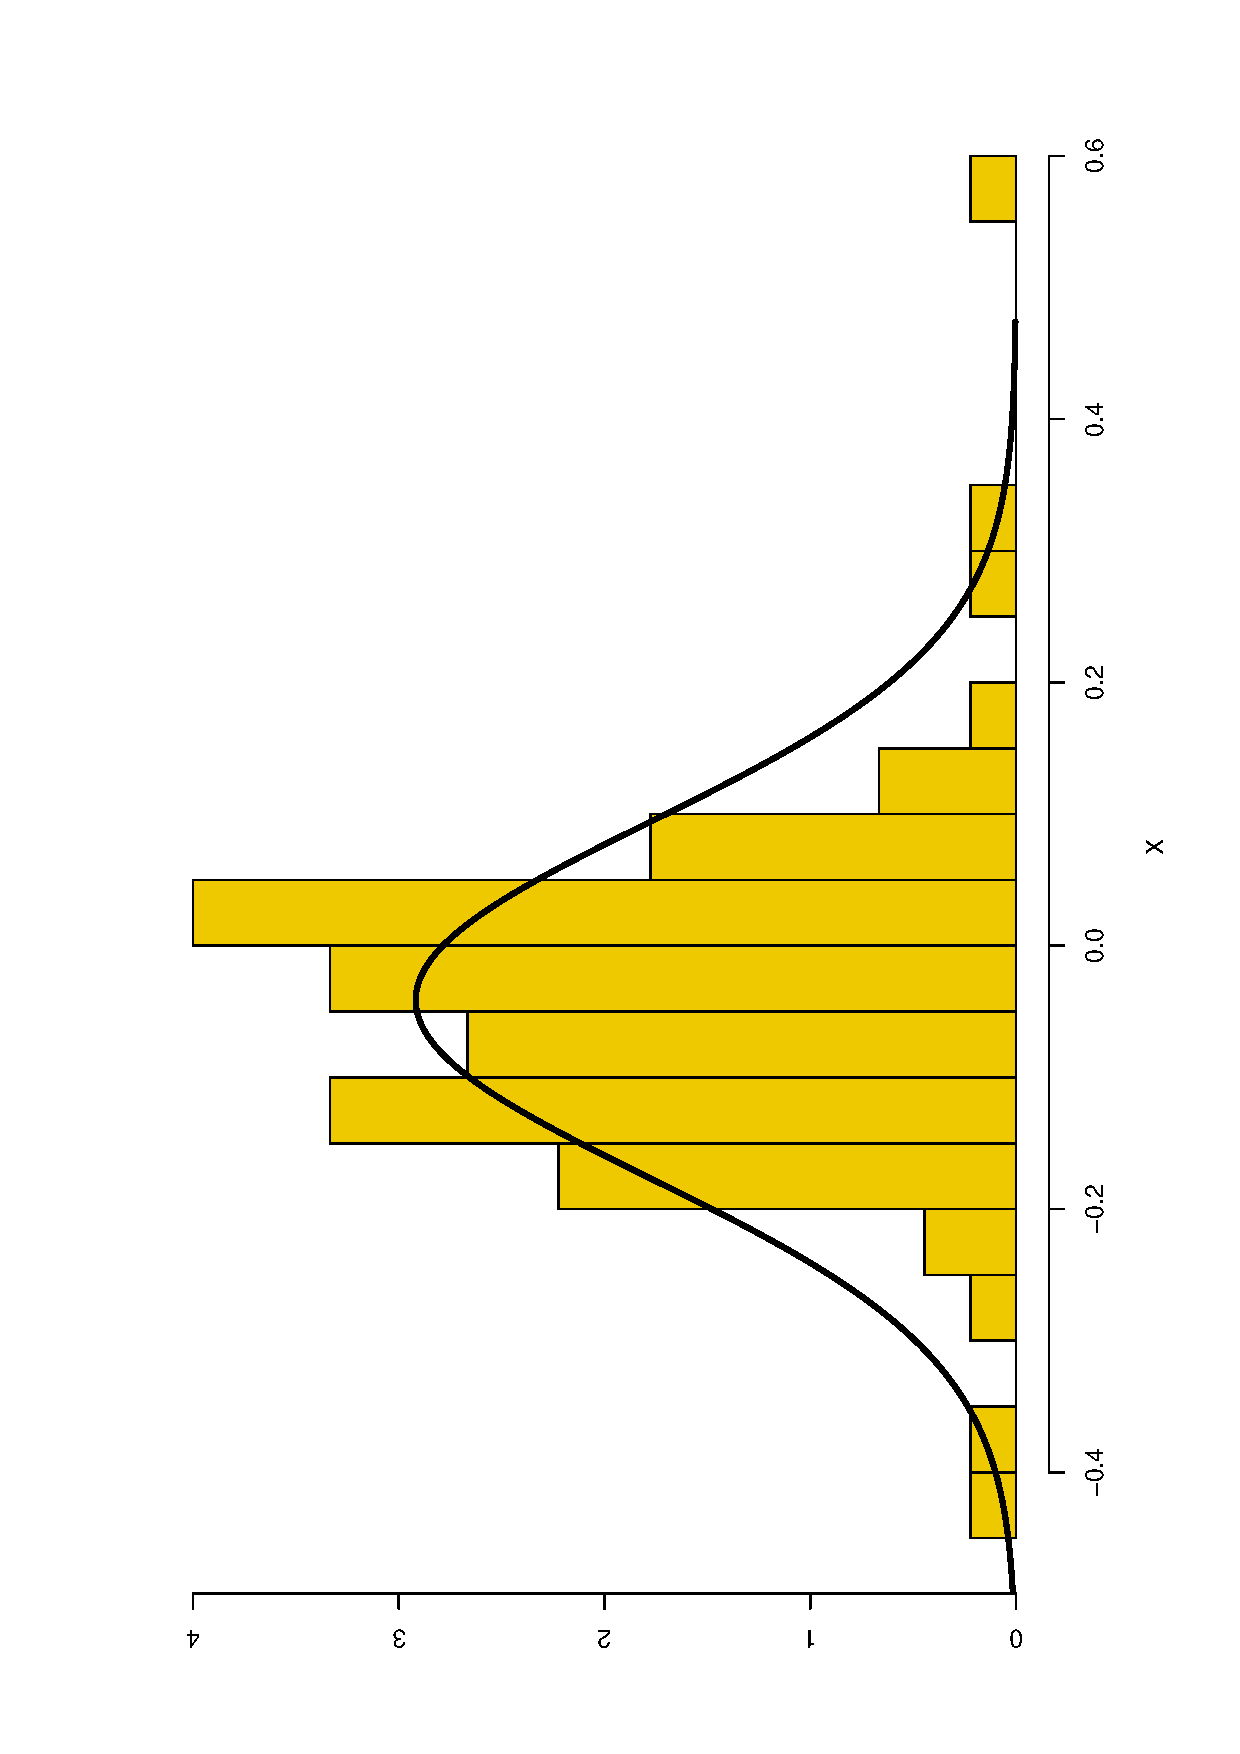
\includegraphics[width=4truecm,angle=270]{figures/predt}
\end{columns}
\end{slide}
